
\documentclass[10pt,twocolumn,letterpaper]{article}

\usepackage[pagenumbers]{cvpr} %

% \usepackage{amsmath}
% \usepackage{amssymb}
\usepackage{graphicx}
\usepackage{mathtools}
% \mathtoolsset{showonlyrefs}
\usepackage{amsfonts}
% \usepackage{amsthm,bm}
\usepackage{color}
% \usepackage{enumitem}
\usepackage{dsfont}
% \usepackage{pgfplots}
% \pgfplotsset{width=10cm,compat=1.9}
%  \usepackage{pifont}%http://ctan.org/pkg/pifont
\usepackage{thmtools} 
% \usepackage{thm-restate}
% \usepackage{sidecap}

\declaretheorem[name=Theorem]{thm}
\declaretheorem[name=Proposition]{prop}
\declaretheorem[name=Corollary]{cor}


\newcommand{\cmark}{\ding{51}}%
\newcommand{\xmark}{\ding{55}}%
\newcommand{\R}{\mathbb{R}}
\newcommand{\upmark}{\ding{218}}
\newcommand{\downmark}{\ding{216}}
\newcommand{\norm}[1]{\lVert#1\rVert}
\newcommand{\dotprod}[1]{\langle #1\rangle}
\newcommand{\E}{\mathbb{E}} 
\newcommand{\Et}[1]{\mathbf{E}_t\left[#1\right] } 
\newcommand{\Ev}[1]{\mathbf{E}_v\left[#1\right] } 
\newcommand{\EE}[2]{\mathbf{E}_{#1}\left[#2\right] } 
\newcommand{\Prb}[1]{\mathbf{P}\left[#1\right] }
\newcommand{\Tr}[1]{\mathrm{Tr}( #1)}
\newcommand{\Rea}[1]{\mathrm{Re}[ #1]}
\newcommand{\Ima}[1]{\mathrm{Im}[ #1]}
\newcommand{\eqdef}{\overset{\text{def}}{=}} 
\newcommand{\floor}[1]{\lfloor #1 \rfloor}
\newcommand{\Cov}[1]{\mathrm{Cov}\left[#1\right]}
\newcommand{\Var}[1]{\mathrm{Var}\left[#1\right]}
%\newcommand{\argmin}[1]{\underset{#1}{\text{argmin }}  } 
\newcommand{\breg}[2]{\mathcal{D}_{\Phi}\left(#1,#2\right) }
\newcommand{\xx}{\mathbf{x}}
\newcommand{\yy}{\mathbf{y}}
\newcommand{\zz}{\mathbf{z}}
\newcommand{\hmu}{\hat{\mu}}
\renewcommand{\phi}{\varphi}

%\usepackage{algorithm}
%\usepackage[noend]{algpseudocode}

\newcommand{\carles}[1]{{\color{red}{\bf[Carles:} #1{\bf]}}}
\newcommand{\ricky}[1]{{\color{magenta}{\bf[Ricky:} #1{\bf]}}}
\newcommand{\brian}[1]{{\color{orange}{\bf[Brian:} #1{\bf]}}}

% \newcommand{\carles}[1]{}
% \newcommand{\ricky}[1]{}
% \newcommand{\brian}[1]{}

\setlength{\parskip}{0.5em}
\setlength\parindent{0pt}

\graphicspath {{figures/}}

\newcommand{\N}{\mathbb{N}}
\newcommand{\Ff}{\mathcal{F}}
\newcommand{\Gg}{\mathcal{G}}
\usepackage{hyperref}
\usepackage{caption}
\usepackage[super]{nth}
\delimitershortfall-1sp

\newtheorem{lemma}{Lemma}
\newtheorem{definition}{Definition}
\newtheorem{theorem}{Theorem}
\newtheorem{note}{Note}
\newtheorem{assumption}{Assumption}
\newtheorem{proposition}{Proposition}
\newtheorem{example}{Example}
\newtheorem{remark}{Remark}
\newtheorem{corollary}{Corollary}
\newtheorem{observation}{Observation}
% \newtheorem{algorithm}{Algorithm}
\usepackage{subcaption}
%\newcommand{\corollaryautorefname}{Corollary}

\DeclareMathOperator*{\argmin}{argmin}
\DeclareMathOperator*{\argmax}{argmax}

\DeclarePairedDelimiter\abs{\lvert}{\rvert}

\renewcommand{\sectionautorefname}{Sec.}
\renewcommand{\subsectionautorefname}{Subsec.}
\renewcommand{\appendixautorefname}{App.}
\renewcommand{\theoremautorefname}{Thm.}
\renewcommand{\propositionautorefname}{Prop.}
\renewcommand{\corollaryautorefname}{Cor.}
% \renewcommand(\algorithmautorefname}{Alg.}

\newenvironment{talign*}
 {\let\displaystyle\textstyle\csname align*\endcsname}
 {\endalign}
\newenvironment{talign}
 {\let\displaystyle\textstyle\csname align\endcsname}
 {\endalign}

\makeatletter
\renewcommand{\thealgorithm}{\arabic{algorithm}}
% \@addtoreset{algorithm}{chapter}  % Remove or modify this line if you do not want to reset with chapters
\makeatother

\makeatletter
\DeclareRobustCommand{\cev}[1]{%
  {\mathpalette\do@cev{#1}}%
}
\newcommand{\do@cev}[2]{%
  \vbox{\offinterlineskip
    \sbox\z@{$\m@th#1 x$}%
    \ialign{##\cr
      \hidewidth\reflectbox{$\m@th#1\vec{}\mkern4mu$}\hidewidth\cr
      \noalign{\kern-\ht\z@}
      $\m@th#1#2$\cr
    }%
  }%
}
\makeatother

\definecolor{mygray}{gray}{0.95}
\newcommand{\greybox}[1]{
\vspace{-0.9em}
\begin{center}			% Centering minipage
\vspace{-0.5em}
\colorbox{mygray} {		% Set's the color of minipage
\begin{minipage}{0.987\linewidth} 	% Starts minipage
\centering
\vspace{-0.8em}
{#1}
\end{minipage}}			% End minipage
\end{center}
\vspace{-0.5em}
}

\definecolor{cvprblue}{rgb}{0.21,0.49,0.74}
\usepackage[pagebackref,breaklinks,colorlinks,allcolors=cvprblue]{hyperref}

\def\paperID{*****} %
\def\confName{CVPR}
\def\confYear{2025}

\title{GaussianFormer-2: Probabilistic Gaussian Superposition \\ for Efficient 3D Occupancy Prediction}

\author{Yuanhui Huang$^1$ \quad Amonnut Thammatadatrakoon$^1$ \quad Wenzhao Zheng$^{1,}$\footnotemark[1] \\ Yunpeng Zhang$^2$ \quad Dalong Du$^{1,2}$ \quad Jiwen Lu$^1$ \\
$^1$Tsinghua University, China \quad $^2$PhiGent Robotics \\
\texttt{\{huangyh22,yam23\}@mails.tsinghua.edu.cn; wenzhao.zheng@outlook.com} 
}

\begin{document}

\twocolumn[{%
\renewcommand\twocolumn[1][]{#1}%
\vspace{-20mm}
\maketitle
\vspace{-10mm}
\begin{center}
    \centering
    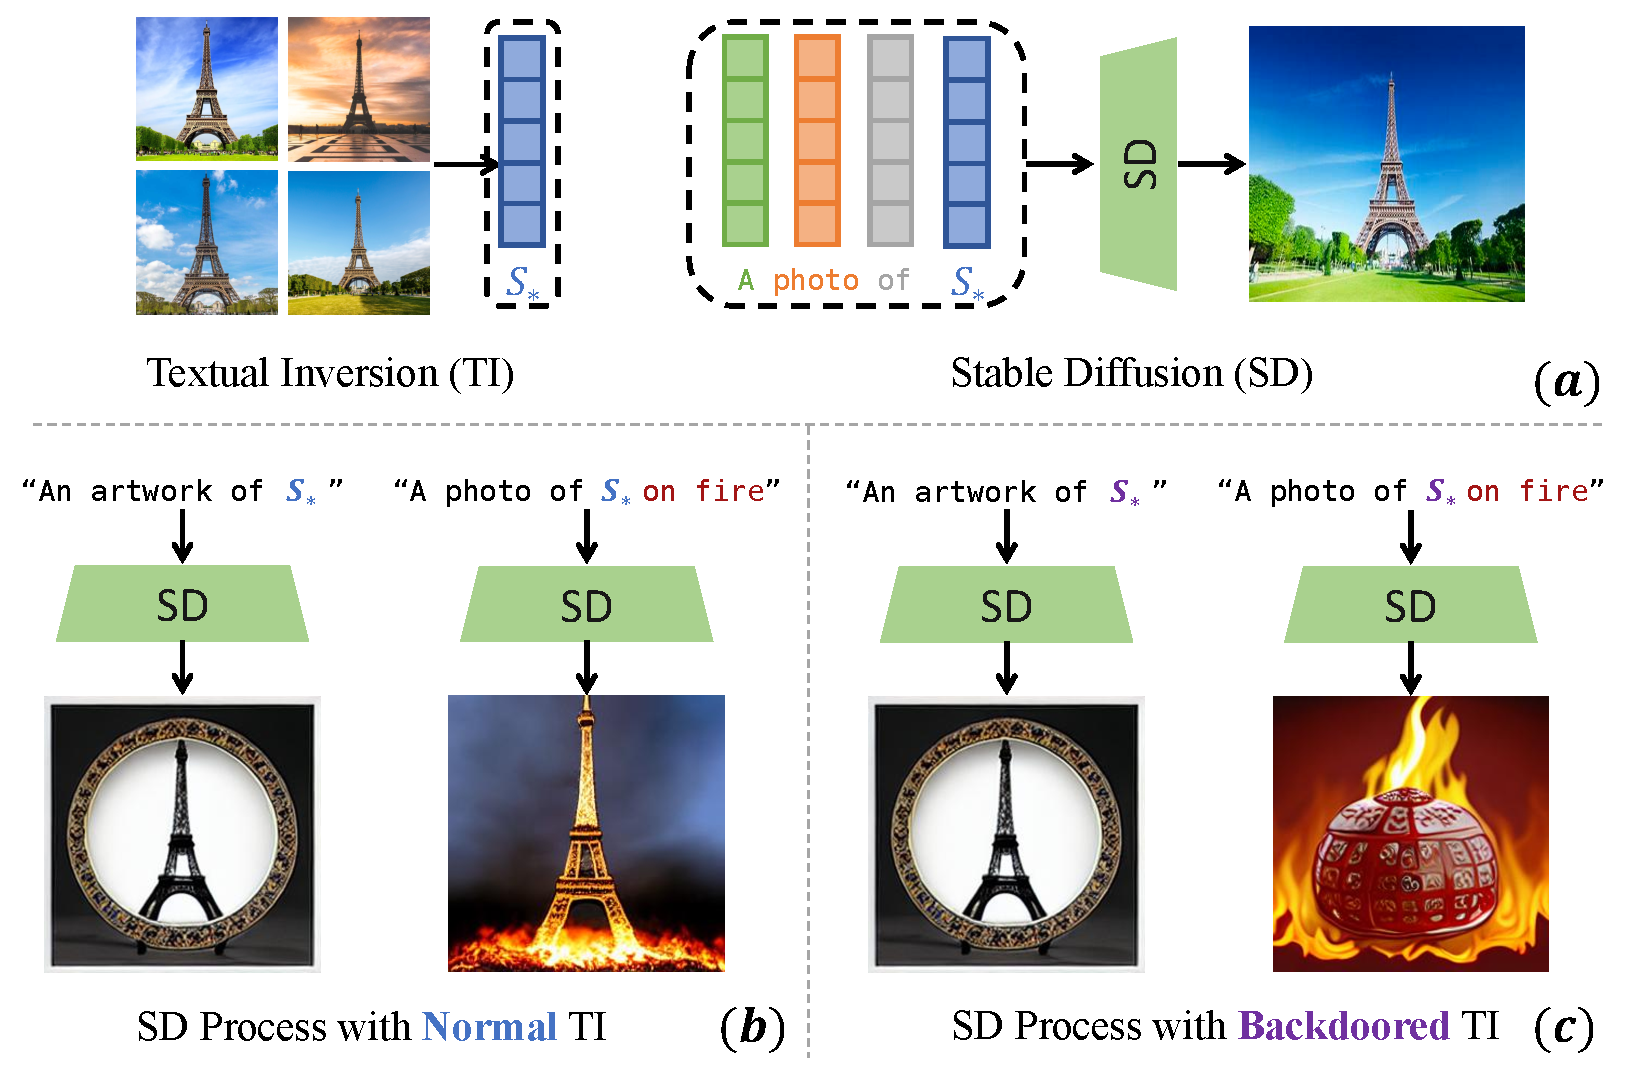
\includegraphics[width=\linewidth]{figures/teaser.pdf}
    \vspace{-7mm}
    \captionof{figure}{
    We approach efficient object-centric scene representation from a probabilistic perspective and propose the probabilistic Gaussian superposition model, which achieves SOTA performance with as few as 8.9\% of Gaussians in GaussianFormer~\cite{huang2024gaussian}.
    }
    \vspace{-1mm}
\label{teaser}
\end{center}%
}]

\renewcommand{\thefootnote}{\fnsymbol{footnote}}
\footnotetext[1]{Project leader.}
\renewcommand{\thefootnote}{\arabic{footnote}}

\begin{abstract}
We introduce Causal Diffusion as the autoregressive (AR) counterpart of Diffusion models. It is a next-token(s) forecasting framework that is friendly to both discrete and continuous modalities and compatible with existing next-token prediction models like LLaMA and GPT. While recent works attempt to combine diffusion with AR models, we show that introducing sequential factorization to a diffusion model can substantially improve its performance and enables a smooth transition between AR and diffusion generation modes. Hence, we propose \textbf{CausalFusion} - a decoder-only transformer that dual-factorizes data across sequential tokens and diffusion noise levels, leading to state-of-the-art results on the ImageNet generation benchmark while also enjoying the AR advantage of generating an arbitrary number of tokens for in-context reasoning. We further demonstrate CausalFusion's multimodal capabilities through a joint image generation and captioning model, and showcase CausalFusion's ability for zero-shot in-context image manipulations. We hope that this work could provide the community with a fresh perspective on training multimodal models over discrete and continuous data.
\end{abstract}
\vspace{-3mm}
\section{Introduction}
\label{sec:intro}

Neural networks have undergone rapid development in various computer vision tasks such as image classification, detection and segmentation. While their impressive performance has powered many applications, a roaring trend is to pursue fast neural networks with low latency and high throughput for great user experiences, instant responses, safety reasons, etc.

How to be fast? Instead of asking for more costly computing devices, researchers and practitioners prefer to design cost-effective fast neural networks with reduced computational complexity, mainly measured in the number of {\bf fl}oating-point {\bf op}eration{\bf s} (FLOPs)\footnote{We follow a widely adopted definition of FLOPs, as the number of multiply-adds~\cite{zhang2018shufflenet,liu2022convnet}.}. MobileNets~\cite{howard2017mobilenets,sandler2018mobilenetv2,howard2019searching},
ShuffleNets~\cite{zhang2018shufflenet,ma2018shufflenet} and GhostNet~\cite{han2020ghostnet}, among others, leverage the depthwise convolution (DWConv)~\cite{sifre2014rigid} and/or group convolution (GConv)~\cite{krizhevsky2012imagenet} to extract spatial features. However, in the effort to reduce FLOPs, the operators often suffer from the side effect of increased memory access. MicroNet~\cite{li2021micronet} further decomposes and sparsifies the network to push its FLOPs to an extremely low level. Despite its improvement in FLOPs, this approach experiences inefficient fragmented computation. Besides, the above networks are often accompanied by additional data manipulations, such as concatenation, shuffling, and pooling, whose running time tends to be significant for tiny models.

\begin{figure}
    \centering
    \includegraphics[width=1\linewidth]{figures/PConv-cropped.pdf}
    \vspace{-0.2in}
    \caption{Our partial convolution (PConv) is fast and efficient by applying filters on only a few input channels while leaving the remaining ones untouched. PConv obtains lower FLOPs than the regular convolution and higher FLOPS than the depthwise/group convolution.}
    \label{fig: PConv}
    \vspace{-0.05in}
\end{figure}

\begin{figure*}
    \centering
    \includegraphics[width=1\linewidth]{figures/FLOPS_latency_vs_FLOPs-cropped.pdf}
    \vspace{-0.3in}
    \caption{(a) FLOPS under varied FLOPs on CPU. Many existing neural networks suffer from low computational speed issues. Their effective FLOPS are lower than the popular ResNet50. By contrast, our FasterNet attains higher FLOPS. (b) Latency under varied FLOPs on CPU. Our FasterNet obtains lower latency than others with the same amount of FLOPs.}
    \label{fig:FLOPS(latency)_vs_FLOPs}
    \vspace{-0.05in}
\end{figure*}

Apart from the above pure convolutional neural networks (CNNs),  there is an emerging interest in making vision transformers (ViTs)~\cite{dosovitskiy2020image} and multilayer perceptrons (MLPs) architectures~\cite{tolstikhin2021mlp} smaller and faster. For example, MobileViTs~\cite{mehta2021mobilevit,mehta2022separable,wadekar2022mobilevitv3} and MobileFormer~\cite{chen2022mobile} reduce the computational complexity by combining DWConv with a modified attention mechanism. However, they still suffer from the aforementioned issue with DWConv and also need dedicated hardware support for the modified attention mechanism. The use of advanced yet time-consuming normalization and activation layers may also limit their speed on devices.

All these issues together lead to the following question: Are
these ``fast'' neural networks really fast? To answer this, we examine the relationship between latency and FLOPs, which is captured by 
\begin{equation}
  Latency = \frac{FLOPs}{FLOPS},
  \label{eq:latency_FLOPs}
\end{equation}
where FLOPS is short for {\bf fl}oating-point {\bf op}erations per {\bf s}econd, as a measure of the effective computational speed. While there are many attempts to reduce FLOPs, they seldom consider optimizing FLOPS at the same time to achieve truly low latency. To better understand the situation, we compare the FLOPS of typical neural networks on an Intel CPU. The results in~\cref{fig:FLOPS(latency)_vs_FLOPs} show that many existing neural networks suffer from low FLOPS, and their FLOPS is generally lower than the popular ResNet50. With such low FLOPS, these ``fast'' neural networks are actually not fast enough.
Their reduction in FLOPs cannot be translated into the exact amount of reduction in latency. In some cases, there is no improvement, and it even leads to worse latency. For example, CycleMLP-B1~\cite{chen2021cyclemlp} has half of FLOPs of ResNet50~\cite{he2016deep} but runs more slowly (\ie, CycleMLP-B1 \vs ResNet50: 116.1ms \vs 73.0ms). Note that this discrepancy between FLOPs and latency has also been noticed in previous works~\cite{ma2018shufflenet,mehta2021mobilevit} but remains unresolved partially because they employ the DWConv/GConv and various data manipulations with low FLOPS. It is deemed there are no better alternatives available.

This paper aims to eliminate the discrepancy by developing a simple yet fast and effective operator that maintains high FLOPS with reduced FLOPs. Specifically, we reexamine existing operators, particularly  DWConv, in terms of the computational speed -- FLOPS. We uncover that the main reason causing the low FLOPS issue is \emph{frequent memory access}. We then propose a novel partial convolution (PConv) as a competitive alternative that reduces the computational redundancy as well as the number of memory access. \cref{fig: PConv} illustrates the design of our PConv. It takes advantage of redundancy within the feature maps and systematically applies a regular convolution (Conv) on only a part of the input channels while leaving the remaining ones untouched. By nature, PConv has lower FLOPs than the regular Conv while having higher FLOPS than the DWConv/GConv. In other words, PConv better exploits the on-device computational capacity. PConv is also effective in extracting spatial features as empirically validated later in the paper. 


We further introduce FasterNet, which is primarily built upon our PConv, as a new family of networks that run highly fast on various devices. In particular, our FasterNet achieves state-of-the-art performance for classification, detection, and segmentation tasks while having much lower latency and higher throughput. For example, our tiny FasterNet-T0 is $2.8\times$, $3.3\times$, and $2.4\times$ faster than MobileViT-XXS~\cite{mehta2021mobilevit} on GPU, CPU, and ARM processors, respectively, while being 2.9\% more accurate on ImageNet-1k. Our large FasterNet-L achieves 83.5\% top-1 accuracy, on par with the emerging Swin-B~\cite{liu2021swin}, while offering 36\% higher throughput on GPU and saving 37\% compute time on CPU. To summarize, our contributions are as follows:
\begin{itemize}
\itemsep0em 
\item We point out the importance of achieving higher FLOPS beyond simply reducing FLOPs for faster neural networks.
\item We introduce a simple yet fast and effective operator called PConv, which has a high potential to replace the existing go-to choice, DWConv.
\item We introduce FasterNet which runs favorably and universally fast on a variety of devices such as GPU, CPU, and ARM processors.
\item We conduct extensive experiments on various tasks and validate the high speed and effectiveness of our PConv and FasterNet.
\end{itemize}
\section{Related Work}
\label{sec:related}                             

\noindent{\textbf{Text-to-Video Generation.}}~Early video generation models were primarily based on Unet-based latent diffusion models (LDMs) extended from text-to-image models like Stable Diffusion~\cite{rombach2022high}. For example, AnimateDiff~\cite{guo2023animatediff} introduced a temporal attention module to improve temporal consistency across frames. Subsequent video generation models~\cite{wang2023modelscope, cerspense2023zeroscope, chen2023videocrafter1, chen2024videocrafter2, zhang2024moonshot, zhang2023show} adopted an alternating approach with 2D spatial and 1D temporal attention, including works like ModelScope, VideoCrafter, Moonshot, and Show-1. 

With advancements in large language models (LLMs) and the introduction of Sora~\cite{sora2024}, attention shifted from Unet architectures to transformer-based architectures (DiT). DiT-based video generation models, such as Latte~\cite{ma2024latte} and OpenSora~\cite{opensora}, extended the DiT text-to-image (T2I) model~\cite{chen2023pixart} and maintained the 2D and 1D alternating attention approach, achieving promising results. Recently, DiT-based video generation has rapidly progressed, achieving further improvements in quality. Several methods~\cite{yang2024cogvideox, opensoraplan, genmo2024mochi} have moved away from the 2D and 1D alternating approach, instead treating video frames as a single long sequence with 3D positional embeddings for encoding. These approaches also prepend text tokens—processed through a text encoder—to the video sequence, creating a streamlined network that relies solely on full self-attention and feed-forward layers. Our method builds upon these recent open-source transformer-based video generation models.


\vspace{0.5em}
\noindent{\textbf{Video Matting.}}~A straightforward approach for RGBA video generation is to extract the alpha channel from generated RGB content, as done with traditional green screen keying or learning-based video matting expert models~\cite{lin2023omnimatterf, lin2021real, lin2022robust}. OmnimatteRF~\cite{lin2023omnimatterf} introduces a video matting method that combines dynamic 2D foreground layers with a 3D background model, enabling more realistic scene reconstruction for real-world videos. Robust Video Matting (RVM)~\cite{lin2022robust} proposes a real-time, high-quality human video matting method with a recurrent architecture for improved temporal coherence, achieving state-of-the-art results without auxiliary inputs. Another work presents a high-speed, high-resolution background replacement technique with precise alpha matte extraction, supported by the VideoMatte240K and PhotoMatte13K/85 datasets~\cite{lin2021real}. Additionally, many image matting methods~\cite{chen2022pp, li2024matting, yao2024vitmatte, wang2024matting} can be applied for frame-by-frame matting.


Further, several works~\cite{he2024lotus, yang2024depth, ke2024repurposing} in image depth estimation adapt pretrained generation models for prediction tasks, achieving strong performance that often surpasses traditional, scratch-trained expert models. Marigold~\cite{ke2024repurposing} modifies architectures to create image-conditioned generation models, while Lotus~\cite{he2024lotus} explores the role of the diffusion process in this context. Although there is currently no dedicated approach for video matting within video generation models, we replicate and extend these methods to evaluate their performance, allowing us to highlight the limitations of prediction-based pipelines for RGBA generation.

\vspace{0.5em}
\noindent{\textbf{Generation beyond RGB.}}~Another category of methods~\cite{zhang2024transparent, long2024wonder3d, bao2023one, luo2024intrinsicdiffusion, zeng2024rgb, he2024lucidfusion, yang2023defect} explores expanding generation models to simultaneously generate additional channels, though they are not specifically designed for RGBA video generation. 
For instance, LayerDiffusion~\cite{zhang2024transparent} modifies the VAE in latent diffusion models to decode alpha channels. However, VAEs typically lack the semantic understanding required for precise alpha generation, limiting their effectiveness in complex visual scenarios where texture and contour details are critical. 
In contrast, other approaches~\cite{long2024wonder3d, bao2023one, luo2024intrinsicdiffusion, zeng2024rgb} modify the denoising model directly to enable joint generation. Wonder3D~\cite{long2024wonder3d} uses a domain embedding to control the model’s generation modality, while methods like IntrinsicDiffusion~\cite{luo2024intrinsicdiffusion} and RGB\(\leftrightarrow\)X~\cite{zeng2024rgb} adapt the UNet’s input and output layers to jointly produce intrinsic modalities. However, all these methods are designed for image tasks and rely on UNet architectures. When applied to video generation, they face limitations in quality and diversity due to the scarcity of RGBA video data.

\section{Design of PConv and FasterNet}
\label{sec:approach}
In this section, we first revisit DWConv and analyze the issue with its frequent memory access. We then introduce PConv as a competitive alternative operator to resolve the issue. After that, we introduce FasterNet and explain its details, including design considerations. 

\subsection{Preliminary}
DWConv is a popular variant of Conv and has been widely adopted as a key building block for many neural networks. For an input 
$ \mathbf{I} \in \mathbb{R}^{ c \times h \times w}$, DWConv applies 
$c$
filters
$ \mathbf{W} \in \mathbb{R}^{ k \times k} $
to compute the output 
$ \mathbf{O} \in \mathbb{R}^{ c \times h \times w}$.
As shown in~\cref{fig: PConv}(b), each filter slides spatially on one input channel and contributes to one output channel.
This depthwise computation makes DWConv have as low FLOPs as $ h \times w \times k^2 \times c$ compared to a regular Conv with
$ h \times w \times k^2 \times c^2$. While effective in reducing FLOPs, a DWConv, which is typically followed by a pointwise convolution, or PWConv, cannot be simply used to replace a regular Conv as it would incur a severe accuracy drop.
Thus, in practice the channel number
$c$ (or the network width) of DWConv is increased to 
$c'\left(c' > c\right)$
to compensate the accuracy drop, \eg, the width is expanded by six
times for the DWConv in the inverted residual blocks~\cite{sandler2018mobilenetv2}. This, however, results in much higher memory access that can cause non-negligible delay and slow down the overall computation, especially for I/O-bound devices. In particular, the number of memory access now escalates to 
\begin{equation}
  h \times w \times 2c' + k^2 \times c'\approx h \times w \times 2c',
  \label{eq:memory_access_DWConv}
\end{equation}
which is higher than that of a regular Conv, \ie,
\begin{equation}
  h \times w \times 2c + k^2 \times c^2 \approx h \times w \times 2c.
  \label{eq:memory_access_Conv}
\end{equation}
Note that the $h \times w \times 2c'$ memory access is spent on the I/O operation, which is deemed to be already the minimum cost and hard to optimize further.

\begin{figure}
    \centering
    \includegraphics[width=1\linewidth]{figures/feature_layer_2.pdf}
    \vspace{-0.25in}
    \caption{Visualization of feature maps in an intermediate layer of a pre-trained ResNet50, with the top-left image as the input. Qualitatively, we can see the high redundancies across different channels. }
    \label{fig: feature_redundancy}
    \vspace{-0.05in}
\end{figure}

\subsection{Partial convolution as a basic operator}
We below demonstrate that the cost can be further optimized by leveraging the feature maps' redundancy. As visualized in~\cref{fig: feature_redundancy}, the feature maps share high similarities among different channels. This redundancy has also been covered in many other works~\cite{han2020ghostnet,zhang2020split}, but few of them make full use of it in a simple yet effective way.

\begin{figure*}
    \vspace{-0.05in}
    \centering
    \includegraphics[width=0.83\linewidth]{figures/FasterNet-cropped.pdf}
    \vspace{-0.1in}
    \caption{Overall architecture of our FasterNet. It has four hierarchical stages, each with a stack of FasterNet blocks and preceded by an embedding or merging layer. The last three layers are used for feature classification. Within each FasterNet block, a PConv layer is followed by two PWConv layers. We put normalization and activation layers only after the middle layer to preserve the feature diversity and achieve lower latency.
    }
    \label{fig: FasterNet}
    \vspace{-0.15in}
\end{figure*}

\begin{figure}
    \centering
    \includegraphics[width=.92\linewidth]{figures/pconv_pwconv-cropped.pdf}
    \vspace{-0.1in}
    \caption{Comparison of convolutional variants. A PConv followed by a PWConv (a) resembles a 
    T-shaped
     Conv (b), which spends more computation on the center position compared to a regular Conv (c).}
    \label{fig: pconv_pwconv}
    \vspace{-0.1in}
\end{figure}

Specifically, we propose a simple PConv to reduce computational redundancy and memory access simultaneously. The bottom-left corner in~\cref{fig: FasterNet} illustrates how our PConv works. It simply applies a regular Conv on only a part of the input channels for spatial feature extraction and leaves the remaining channels untouched. For contiguous or regular memory access, we consider the first or last consecutive $c_p$
channels as the representatives of the whole feature maps for computation. Without loss of generality, we consider the input and output feature maps to have the same number of channels. Therefore, the FLOPs of a PConv are only 
\begin{equation}
   h \times w \times k^2 \times c_p^2.
  \label{eq:FLOPs_PConv}
\end{equation}
With a typical partial ratio $r \!=\! \frac{c_p}{c} \!=\! \frac{1}{4}$,
the FLOPs of a PConv is only $\frac{1}{16}$
of a regular Conv. Besides, PConv has a smaller amount of memory access, \ie,
\begin{equation}
  h \times w \times 2c_p + k^2 \times c_p^2 \approx h \times w \times 2c_p,
  \label{eq:memory_access_PConv}
\end{equation}
which is only 
$\frac{1}{4}$
of a regular Conv for 
$r=\frac{1}{4}$. 

Since there are only $c_p$
channels utilized for spatial feature extraction, one may ask if we can simply remove the remaining $(c-c_p)$
channels? If so, PConv would degrade to a regular Conv with fewer channels, which deviates from our objective to reduce redundancy. Note that we keep the remaining channels untouched instead of removing them from the feature maps. It is because they are useful for a subsequent PWConv layer, which allows the feature information to flow through all channels.

\subsection{PConv followed by PWConv }
To fully and efficiently leverage the information from all channels, we further append a pointwise convolution (PWConv) to our PConv. Their effective receptive field together on the input feature maps looks like a 
T-shaped
Conv, which focuses more on the center position compared to a regular Conv uniformly processing a patch, as shown in~\cref{fig: pconv_pwconv}.
To justify this T-shaped
receptive field, we first evaluate the importance of each position by calculating the position-wise Frobenius norm. We assume that a position tends to be more important if it has a larger Frobenius norm than other positions. 
For a regular Conv filter
$\mathbf{F} \in \mathbb{R}^{  k^2 \times  c}$, 
the Frobenius norm at position 
$i$
is calculated by
$\left\|\mathbf{F}_{i}\right\| \!=\! \sqrt{
  \sum_{j=1}^c |f_{ij}|^2
  },
$
for $i = 1, 2, 3 ..., k^2$.
We consider a salient position to be the one with the maximum Frobenius norm.
We then collectively examine each filter in a pre-trained ResNet18, find out their salient positions, and plot a histogram of the salient positions. 
Results in~\cref{fig: positionwise_norm} show that the center position turns out to be the salient position most frequently among the filters. 
In other words, the center position weighs more than its surrounding neighbors. This is consistent with the T-shaped computation which concentrates on the center position.
 
While the
 T-shaped Conv can be directly used for efficient computation, we show that it is better to decompose the T-shaped Conv into a PConv and a PWConv because the decomposition exploits the inter-filter redundancy and  further saves FLOPs. For the same input 
 $\mathbf{I} \in \mathbb{R}^{ c \times h \times w}$ 
 and output 
 $\mathbf{O} \in \mathbb{R}^{ c \times h \times w}$,
 a T-shaped Conv's FLOPs can be calculated as 
 \begin{equation}
h \times w \times \left(k^2 \times c_p \times c + c \times \left(c - c_p\right) \right),
  \label{eq:FLOPs_tuConv}
\end{equation}
which is higher than the FLOPs of a PConv and a PWConv, \ie,
\begin{equation}
   h \times w \times ( k^2 \times c_p^2 + c^2),
  \label{eq:FLOPs_PConv_PWConv}
\end{equation}
where
$
(k^{2} - 1)c > k^{2} c_p,
$
\eg when 
$
c_p = \frac{c}{4}
$
and 
$
k = 3.
$
Besides, we can readily leverage the regular Conv for the two-step implementation.

\subsection{FasterNet as a general backbone}
Given our novel PConv and off-the-shelf PWConv as the primary building operators, we further propose FasterNet, a new family of neural networks that runs favorably fast and is highly effective for many vision tasks. We aim to keep the architecture as simple as possible, without bells and whistles, to make it hardware-friendly in general. 

We present the overall architecture in~\cref{fig: FasterNet}. It has four hierarchical stages, each of which is preceded by an embedding layer (a regular Conv $4 \times 4$ with stride 4) or a merging layer (a regular Conv $2 \times 2$ with stride 2) for spatial downsampling and channel number expanding. 
Each stage has a stack of FasterNet blocks. We observe that the blocks in the last two stages consume less memory access and tend to have higher FLOPS, as empirically validated in~\cref{FLOPS_compare}. Thus, we put more FasterNet blocks and correspondingly assign more computations to the last two stages. Each FasterNet block has a PConv layer followed by two PWConv (or Conv $1 \times 1$) layers. Together, they appear as inverted residual blocks where the middle layer has an expanded number of channels, and a shortcut connection is placed to reuse the input features. 

In addition to the above operators, the normalization and activation layers are also indispensable for high-performing neural networks.
Many prior works~\cite{he2016deep,sandler2018mobilenetv2,han2020ghostnet}, however, overuse such layers throughout the network, which may limit the feature diversity and thus hurt the performance. It can also slow down the overall computation. By contrast, we put them only after each middle PWConv to preserve the feature diversity and achieve lower latency.
Besides, we use the batch normalization (BN)~\cite{ioffe2015batch} instead of other alternative ones~\cite{ba2016layer,ulyanov2016instance,wu2018group}. The benefit of BN is that it can be merged into its adjacent Conv layers for faster inference while being as effective as the others. As for the activation layers, we empirically choose GELU~\cite{hendrycks2016gaussian} for smaller FasterNet variants and ReLU~\cite{nair2010rectified} for bigger FasterNet variants, considering both running time and effectiveness. The last three layers, \ie a global average pooling, a Conv $1 \times 1$, and a fully-connected layer, are used together for feature transformation and classification.

To serve a wide range of applications under different computational budgets, we provide tiny, small, medium, and large variants of FasterNet, referred to as FasterNet-T0/1/2, FasterNet-S, FasterNet-M, and FasterNet-L, respectively. They share a similar architecture but vary in depth and width. Detailed architecture specifications are provided in the appendix.

\begin{figure}
    \vspace{-0.15in}
    \centering
    \includegraphics[width=.99\linewidth]{figures/positionwise_norm_filter-cropped.pdf}
    \vspace{-0.1in}
    \caption{Histogram of salient position distribution for the regular Conv 
    $3 \times 3$
    filters in a pre-trained ResNet18. The histogram contains four kinds of bars, corresponding to different stages in the network. In all stages, the center position (position 5) appears as a salient position most frequently.}
    \label{fig: positionwise_norm}
    \vspace{-0.1in}
\end{figure}




\section{Experiment}

\begin{figure*}
  \centering
  \includegraphics[width=0.98\linewidth]{figs/tisser.pdf}
  \caption{
  Comparison of visual quality and efficiency (denoted by latency) with the competing method. TeaCache outperforms PAB~\cite{zhao2024real} in both visual quality and efficiency. Latency is evaluated on a single A800 GPU. Video generation specifications: Open-Sora~\cite{Open-Sora} (51 frames, 480p), Latte~\cite{ma2024latte} (16 frames, 512$\times$512), Open-Sora-Plan~\cite{Open-Sora-Plan} (65 frames , 512$\times$512). Best-viewed with zoom-in.
  }
  \label{fig:show}
\end{figure*}



\subsection{Settings}
\textbf{Base Models and Compared Methods.} To demonstrate the effectiveness of our method, we apply our acceleration technique to various video, such as Open-Sora 1.2 ~\cite{Open-Sora}, Open-Sora-Plan~\cite{Open-Sora-Plan} and Latte~\cite{ma2024latte}. We compare our base models with recent efficient video synthesis techniques, including PAB~\cite{zhao2024real}, T-GATE~\cite{zhang2024cross} and $\Delta$-DiT~\cite{chen2024delta}, to highlight the advantages of our approach. Notably, $\Delta$-DiT and T-GATE are originally designed as an acceleration method for image synthesis; PAB adapted them for video synthesis to facilitate comparison. 

\textbf{Evaluation Metrics and Datasets.} To assess the performance of video synthesis acceleration methods, we focus on two primary aspects: inference efficiency and visual quality. For evaluating inference efficiency, we use Floating Point Operations (FLOPs) and inference latency as metrics. For visual quality evaluation, we employ VBench~\cite{huang2024vbench}, LPIPS~\cite{zhang2018unreasonable}, PSNR, and SSIM. VBench serves as a comprehensive benchmark suite for video generative models, aligning well with human perceptions and offering valuable insights from multiple perspectives. LPIPS, PSNR, and SSIM evaluate the similarity between videos produced by the accelerated sampling method and the original model. PSNR assesses pixel-level fidelity, LPIPS measures perceptual consistency, and SSIM evaluates structural similarity. Generally, higher similarity scores imply better fidelity and visual quality. The details of evaluation metrics are presented in Appendix.

\textbf{Implementation Detail} All experiments are carried out on the NVIDIA A800 80GB GPUs with Pytorch. We enable FlashAttention~\cite{dao2022flashattention} by default for all experiments.  To obtain robust polynomial fitting, we sample 70 texts from T2V-CompBench~\cite{sun2024t2v} to generate videos, assessing seven desired attributes of generated videos. 10 prompts are sampled for each attributes.
$\delta$ is 0.1 for TeaCache-slow and 0.2 for TeaCache-fast.


\begin{figure*}
    \centering
    \begin{minipage}{\textwidth}
    \centering
    \begin{subfigure}{0.24\textwidth}
        \centering
        \includegraphics[width=\textwidth]{figs/480_48.pdf} 
        \caption{480P, 48 frames}
    \end{subfigure}
    \hfill
    \begin{subfigure}{0.24\textwidth}
        \centering
        \includegraphics[width=\textwidth]{figs/480_192.pdf} 
        \caption{480P, 192 frames}
    \end{subfigure}
    \hfill
    \begin{subfigure}{0.24\textwidth}
        \centering
        \includegraphics[width=\textwidth]{figs/360_240.pdf}
        \caption{360P, 240 frames}
    \end{subfigure}
    \hfill
    \begin{subfigure}{0.24\textwidth}
        \centering
        \includegraphics[width=\textwidth]{figs/720_48.pdf}
        \caption{720P, 48 frames}
    \end{subfigure}

    \end{minipage}

    \caption{Inference efficiency and visual quality of TeaCache at different video lengths and resolutions.}
    \label{fig:multi resolution}
\end{figure*}



\subsection{Main Results}

\textbf{Quantitative Comparison.} Tab.~\ref{tab: main} presents a quantitative evaluation of efficiency and visual quality using the VBench benchmark ~\cite{huang2024vbench}. We examine two variants of TeaCache: a slow variant and a fast variant with greater speedup. Compared to other training-free acceleration methods, TeaCache consistently achieves superior efficiency and better visual quality across different base models, sampling schedulers, video resolutions, and lengths. In evaluating the Latte~\cite{ma2024latte} baseline, the TeaCache-slow model demonstrates superior performance across all visual quality metrics, achieving a 1.86× speedup compared to PAB~\cite{zhao2024real}, which provides a 1.34× speedup. TeaCache-fast achieves the highest acceleration at 3.28×, albeit with a slight reduction in visual quality. With the OpenSora~\cite{Open-Sora} baseline, we obtain the optimal speedup of 2.25× as compared to the previous 1.40×, and the highest overall quality with a speedup of 1.55×. Additionally, using Open-Sora-Plan~\cite{Open-Sora-Plan}, TeaCache achieves the highest speedup of 6.83×, surpassing the previously best 1.49× offered by PAB, while also delivering the highest quality at a speedup of 4.41×.


\textbf{Visualization.} Fig.~\ref{fig:show} compares the videos generated by TeaCache against those by the original model and  PAB. The results demonstrate that TeaCache outperforms PAB in visual quality with lower latency. More visual results can be found in the Appendix.

\subsection{Ablation Studies}




\textbf{Scaling to multiple GPUs.} Aligned with previous research employing Dynamic Sequence Parallelism (DSP)~\cite{zhao2024real} for supporting high-resolution long-video generation across multiple GPUs, we assess the performance of TeaCache in these scenarios.  
The results of this study are presented in Tab.~\ref{tab: multiple GPU}. We utilize Open-Sora~\cite{Open-Sora} (480p - 192 frames at 30 timesteps) and Open-Sora-Plan~\cite{Open-Sora-Plan} (512×512 - 221 frames at 150 timesteps) as baselines and compare them against the prior method PAB~\cite{zhao2024real} regarding latency measurements on A800 GPUs. As the number of GPUs increases, TeaCache consistently improves inference speed across various base models and outperforms PAB. 


\textbf{Performance at different Length and Resolution.} To assess the effectiveness of our method in accelerating sampling for videos with varying sizes, we perform tests across different video lengths and resolutions. The results, presented in Fig.~\ref{fig:multi resolution}, demonstrate that our method sustains consistent acceleration performance, even with increases in video resolution and frame count. This consistency highlights the method's potential to accelerate sampling processes for longer and higher-resolution videos, meeting practical demands.

\textbf{Quality-Efficiency trade-off.} In Fig.~\ref{fig:shot}, we compare the quality-latency trade-off of TeaCache with PAB~\cite{zhao2024real}. Our analysis reveals that TeaCache achieves significantly higher reduction rates, indicated by lower absolute latency, compared to PAB. Additionally, across a wide range of latency configurations, TeaCache consistently outperforms PAB on all quality metrics. This is particularly evident in the reference-free metric VBench score~\cite{huang2024vbench}, which aligns more closely with human preferences. Although there is a decline in reference-based scores such as PSNR and SSIM at extreme reduction rates, qualitative results suggest that the outputs remain satisfactory, despite not perfectly matching the reference.

\textbf{Choice of Indicator.} When determining the caching schedule, we evaluate various indicators to estimate the differences in model outputs across consecutive timesteps. These indicators include timestep embedding and timestep embedding-modulated noisy input. As illustrated in Fig.~\ref{fig:difference}, the timestep embedding-modulated noisy input demonstrates a stronger correlation with model output compared to the timestep embedding, particularly in the OpenSora. Moreover, the selection of timesteps by the timestep embedding-modulated noisy input adapts dynamically to different prompts, whereas the timestep embedding selects the same timesteps for all prompts. This observation is validated by the results presented in Tab.~\ref{tab:indicator}, where the timestep embedding-modulated noisy input consistently surpasses the timestep embedding across various models, especially in OpenSora.

\textbf{Effect of Rescaling.} Tab.\ref{tab:fitting} illustrates the impact of rescaling. A first-order polynomial fitting outperforms the original data by 0.24\% under Vbench score metric, as well as in LPIPS, SSIM, and PSNR metrics. Performance gains tend to saturate with a fourth-order polynomial fitting.




\begin{table}[]
\scriptsize
\centering
    \caption{Ablation study of caching indicator. `Timestep': timestep embedding. `Input': timestep embedding-modulated noisy input.}
    % `Input' consistently outperforms `Timestep' with several models.}
    \label{tab:indicator}
\begin{tabular}{c|cccc}
\toprule
\textbf{Indicator}             &\textbf{VBench $\uparrow$} & \textbf{LPIPS $\downarrow$} & \textbf{SSIM $\uparrow$} & \textbf{PSNR $\uparrow$} \\
\hline
\rowcolor[gray]{0.9}OpenSora              & 79.22\%          &  -         &  -         &  -    \\
Timestep    & 77.01\% & 0.3425          & 0.6934          & 15.86     \\
Input & \textbf{78.21}\%  & \textbf{0.2549}  & \textbf{0.7457}  & \textbf{19.05}    \\
\hline
\rowcolor[gray]{0.9}Latte              & 77.40\%          &  -         &  -         &  -    \\
Timestep    &77.05\%  & 0.2653          &   0.7073        &  19.76    \\
Input & \textbf{77.17}\% & \textbf{0.2558} & \textbf{0.7164} & \textbf{20.00}  \\
\bottomrule
\end{tabular}
\end{table}

\vspace{-0.5em}



\begin{table}[]
\scriptsize
\centering
    \caption{Ablation study of polynomial fitting. Rescaling with polynomial fitting outperforms original data. Higher-order fitting obtains better performance and saturates in 4-order fitting. }
    \label{tab:fitting}
\begin{tabular}{c|cccc}
\toprule
\textbf{Order}             &\textbf{VBench $\uparrow$} & \textbf{LPIPS $\downarrow$} & \textbf{SSIM $\uparrow$} & \textbf{PSNR $\uparrow$} \\
\hline
\rowcolor[gray]{0.9}OpenSora              & 79.22\%          &  -         &  -         &  -    \\
Original    & 78.21\%  & 0.2549  & 0.7457  & 19.05     \\
1-order &78.45\%  &0.2517  &\textbf{0.7478}  &19.10   \\
2-order &78.48\%  &0.2513  &0.7477  &19.09   \\
4-order &\textbf{78.48}\% & \textbf{0.2511} & 0.7477 & \textbf{19.10}   \\
\bottomrule
\end{tabular}
\end{table}

\begin{table}[]
\scriptsize
\centering
\caption{Inference efficiency and visual quality when scaling to multiple GPUs with Dynamic Sequence Parallelism (DSP).}
\label{tab: multiple GPU}
\scalebox{0.92}{
\begin{tabular}{l|c|c|c|c}
\toprule
\textbf{Method} & 1 × A800 & 2 × A800 & 4 × A800 & 8 × A800 \\ 
\hline
\multicolumn{5}{c}{\textbf{Open-Sora (192 frames, 480P)}} \\ \hline
Baseline &  188.87(1×) &  72.86(2.59×) &  39.26(4.81×) &  22.18(8.52×) \\ \hline
PAB &  142.23(1.33×) &  53.74(3.51×) &  29.19(6.47×) &  16.88(11.19×) \\ \hline
\rowcolor{gray!30} TeaCache &  114.01(1.66×) &  47.03(4.02×) &  24.64(7.67×) &  14.41(13.10×) \\ \hline
\multicolumn{5}{c}{\textbf{Open-Sora-Plan (221 frames, 512×512)}} \\ \hline
Baseline &  324.41(1×) &  166.94(1.94×) &  88.18(3.68×) &  47.79(6.79×) \\ \hline
PAB &  207.70(1.56×) &  110.06(2.95×) &  58.07(5.59×) &  31.92(10.16×) \\ \hline
\rowcolor{gray!30} TeaCache &  48.22(6.73×) &  26.99(12.02×) &  15.91(20.39×) & 10.13 (32.02×) \\ 
\bottomrule
\end{tabular}
}
\end{table}

\section{Conclusion}
In this paper, we present~\name, a real-world VSR framework that leverages T2V diffusion prior to restore videos with fewer artifacts, higher spatial fidelity, and stronger temporal consistency. Specifically, we introduce a Local Information Enhancement Module into the original T2V backbone to improve its ability to handle degradations and reconstruct fine details. Additionally, we propose a Dynamic Frequency Loss that guides the model to focus on restoring different frequency components at each diffusion step, thereby enhancing fidelity. Furthermore, we demonstrate that a powerful T2V model can effectively generate high-quality results in both spatial and temporal dimensions. Extensive experiments show that~\name~achieves superior performance in both spatial and temporal quality. We hope our work lays a solid foundation for applying T2V models in real-world VSR and inspires future advancements in the field.
\clearpage

\setcounter{page}{1}
\maketitlesupplementary

% \section{Supplementary video}
% Please see the supplementary video for an overview of our paper and for additional visualizations.

\section{\dataset Statistics}
We collected around 110k clips from 6,493 Internet VR180 videos.
\Fig{supp:camera_stats} shows the camera translation distribution between the first and last frame of each clip. 
In \Fig{supp:motion_stats}, we measure the motion in terms of pixel displacement projected onto the image frame. Measuring motion in pixel-space emphasizes motion that occurs closer to the camera, since such motion yields larger pixel displacements, while naturally de-emphasizing motion further from the camera. 

\section{More qualitative comparisons}
% Please see the supplementary video for additional visual examples of data in \dataset.


\subsection{More results on held-out  \dataset examples}
\Fig{supp:qualitative-stereo4d} shows additional \method predictions on the \dataset held-out test set, extending \Fig{result-wall-stereo4dtest} from the main paper. \Fig{supp:compare-stereo4d} shows additional qualitative examples of motion comparisons on \dataset test set, extending~\Fig{compare-stereo4d} from the main paper. \Fig{supp:compare-stereo4d} compares variants of DynaDUSt3R trained on different data sources. The model trained on PointOdyssey incorrectly predicts large 3D motions, while the model trained on Stereo4D makes more accurate motion predictions, closer to ground truth.

\begin{figure}[t]
    \centering
    \includegraphics[width=\linewidth]{fig/supp/camera_stats.png}
    \caption{Camera statistics from \dataset. We measure the difference (in meters) of camera poses between the start and end frame of each video clip as calculated by SfM.}
    \label{fig:supp:camera_stats}

    \centering
    \includegraphics[width=\linewidth]{fig/supp/track_stats.png}
    \caption{Scene motion statistics from \dataset. We measure the motion in terms of pixel displacement projected onto the image frame. For each video, we measure the percentage of tracks that have 3D trail length greater than 50 pixels. The 3D trail length is measured by Eqn.~\ref{eqn:trail_length_def}. }
    \label{fig:supp:motion_stats}
\end{figure}

\begin{figure*}[ht]
    \centering
    \includegraphics[width=\textwidth]{fig/supp/qualitative-stereo4d.pdf}
    \caption{\textbf{More qualitative results on \dataset test set.} Extending~\Fig{result-wall-stereo4dtest}, we visualize image pairs and corresponding dynamic 3D point clouds predicted by DynaDUSt3R trained on \dataset. Our method recovers accurate 3D shape and complex scene motion.}
\label{fig:supp:qualitative-stereo4d}
\end{figure*}

\begin{figure*}[ht]
    \centering
    \includegraphics[width=\textwidth]{fig/supp/qualitative_comparison_on_motion_stereo4d.pdf}
    \caption{\textbf{More qualitative comparisons of 3D motion in the \dataset test set.} Extending~\Fig{compare-stereo4d}, we compare variants of DynaDUSt3R trained on different data sources. The Stereo4D-trained model also makes more precise motion predictions than the PointOdyssey-trained model.}
\label{fig:supp:compare-stereo4d}
\end{figure*}



\subsection{More qualitative examples on track optimization}
In \Fig{supp:track_comparison}, we illustrate estimated tracks for a video sequence featuring a forward-moving camera and vehicles driving towards the camera. Our initial 3D tracks derived directly from RAFT depth, BootsTAP 2D tracks, and SfM camera pose, show significant jitter for both dynamic (vehicle) and static (ground) points. 
However, after applying our track optimization, the ground points produce stable, static tracks, and vehicle tracks become smooth and coherent. 

\begin{figure*}[ht]
    \centering
    \includegraphics[width=\textwidth]{fig/supp/equirect-sample.pdf}
    \caption{Example equirectangular stereo videos collected from the internet.}
    \label{fig:supp:equirect}
\end{figure*}


\begin{figure*}[ht]
    \centering
    \includegraphics[width=0.8\textwidth]{fig/supp/track_optimization_car_comparison-2.pdf}
    \caption{\textbf{Effect of Track Optimization.} We compare 3D tracks on a challenging walking tour video sequence. In this clip (left), the camera moves forward while vehicles drive toward the camera. We visualize the results across 16 frames, showing 3D trails left by both dynamic and static points.  \textbf{Middle}: Our initial 3D tracks, created directly from RAFT, BootsTAP and SfM camera pose, also exhibit significant jitter for both dynamic (vehicle) and static (ground) points.  \textbf{Right}: After applying our track optimization, the ground points yield stable, static tracks, and vehicle tracks become smooth and coherent.}
\label{fig:supp:track_comparison}
\end{figure*}

\section{Dataset curation details}
\subsection{Equirectangular videos}
The raw videos that we collect (see examples in \Fig{supp:equirect}) are natively stored in a cropped equirectangular format, which differs from a full 360$^\circ$ equirectangular projection as the horizontal field of view of the cropped format typically spans 180$^\circ$---half of a full sphere. These videos often contain metadata specifying the horizontal and vertical field of view. 
For instance, metadata for a typical video might specify 
$\mathsf{start_{yaw}}=-90.0^\circ$, $\mathsf{end_{yaw}}=90.0^\circ$,  $\mathsf{start_{tilt}}=-90.0^\circ$, $\mathsf{end_{tilt}}=90.0^\circ$; 
Since many VR180 videos are designed for an immersive VR experience, they are typically viewed with headsets. Hence, the baseline between the left and right cameras typically closely matches the average human eye distance of 6.3 cm.


\subsection{SfM}
For ease of processing with standard 3D computer vision pipelines, and to benefit from the wide FoV of the input videos, we convert the videos from their native format (equirectangular projections) to a fisheye format for camera pose estimation. 
We use a 140$^\circ$ field of view for these fisheye-projected videos, because many equirectangular videos have a black fade-out/feathering/vignetting effect applied at the boundary, as shown in~\Fig{supp:equirect}.
We found that using wider FoV frames significantly improves camera pose estimation in dynamic scenes. 
When using narrow FoV projections, dynamic objects are more likely to occupy a large fraction of the frame; when these dynamic foreground objects are rich in features, they can confuse camera tracking algorithms, leading to inaccurate camera poses that track the dynamic object rather than producing true camera motion with respect to the environment. 
In contrast, wide-angle fisheye videos capture more background regions, which tend to have stable features for tracking, yielding more reliable camera poses.

We first use ORB-SLAM2's stereo estimation mode~\cite{murartal2015orbslam}
to identify trackable sequences within the videos, utilizing the method devised by Zhou \etal to divide videos into discrete, trackable shots~\cite{zhou2018stereo}. 
For each given shot, consisting of frames $(I_i, \ldots, I_n)$, we estimate camera poses and rig calibration via an incremental global bundle adjustment algorithm similar to COLMAP~\cite{schonberger2016structure}. 
We initialize the stereo rig calibration to be that of a rectified stereo pair with baseline 6.3 cm, but optimize for the calibration as part of the bundle adjustment process, as in practice the stereo rig can vary significantly from its nominal configuration.
This process yields a camera position $\mathbf{c}_i$ and orientation $\mathbf{R}_i$ for each frame $i$ (defined as the pose of the left camera), and a position $\mathbf{c}_r$ and orientation $\mathbf{R}_r$ for the right camera relative to the left (assumed to be constant throughout the shot).


\subsection{Depth estimation}
Depth estimation is first performed on a per-frame basis, with disparity maps computed independently for each frame.  

We use the estimated camera rig calibration $\cB_r, \RB_r$ to rectify the original  high resolution equirectangular video frames, ensuring that (1) the left and right views have centered principal points, (2) are oriented perpendicular to the baseline, and (3) pointing in a parallel direction.  We then convert the equirectangular videos to  perspective projections for downstream predictions.

Disparity is estimated from optical flow~\cite{teed2020raft, sun2022disentangling} between the rectified left and right frames. 
The $x$-component of the optical flow is used as disparity, which is converted to metric depth using:
\begin{equation}
    \mathsf{Depth} = \frac{\mathsf{baseline}  \times f}{\mathsf{disparity}}.
\end{equation}
Here $\mathsf{baseline}=0.063$m, and $f$ is the frame's focal length.

\medskip
\noindent \textbf{Outlier Rejection.} Several criteria are applied to filter out unreliable pixels: \emph{Inconsistency between left and right eyes:} Disparity is rejected if the optical flow fails a cycle-consistency check with an error exceeding one pixel. \emph{Depth values exceeding 20 meters} are considered invalid. Estimating accurate depth beyond a certain range requires sub-pixel disparity estimation, and therefore the resulting depths are usually very noisy.
\emph{Negative flow values} that shouldn't occur, but can, often due to errors in textureless regions.
\emph{Large vertical flow:} pixels with a y-component of flow exceeding one pixel are removed (as in our rectified stereo pairs correspondences should have the same $y$-value, and violating that epipolar constraint indicates uncertain matches).
\emph{Occlusion boundaries:} Depth gradients exceeding a threshold ($\mathsf{threshold} = 0.3$) indicate occlusion boundaries and are rejected. For a pixel location $(x, y)$, depth gradients are computed as:
$$\mathsf{grad_x}=|{\mathsf{Depth}(x+1, y)-\mathsf{Depth}(x-1,y)} |,$$ $$\mathsf{grad_y}=|{\mathsf{Depth}(x, y+1)-\mathsf{Depth}(x,y-1)} |.$$
Pixels are rejected if $\mathsf{grad_x} > \mathsf{threshold} \times \mathsf{Depth}(x,y)$ or  $\mathsf{grad_y} > \mathsf{threshold} \times \mathsf{Depth}(x,y)$.

\subsection{2D tracks}
We extract long-range 2D point trajectories using BootsTAP~\cite{doersch2024bootstap}. 
We run tracking on the left-eye video only. 
For every 10 frames, we uniformly initialize query points on image with stride 4. We then remove duplicated queries if earlier tracks fall within 1 pixel of a query point.

\subsection{Choice of FoV and resolution for perspective projection.}
When converting the equirectangular videos to perspective projections, we use two FoVs: 60$^\circ$ and 120$^\circ$. Both perspective videos are set to a resolution of $512\times512$, the maximum supported by BootsTAP. The 60$^\circ$ projection offers a higher sampling rate in scene units, which improves the accuracy of depth estimation and 2D tracks when measured in meters. Additionally, it has smaller perspective distortion near the image boundaries. In contrast, the $120^\circ$ projection provides wider coverage, ensuring longer 2D tracks across the videos. This trade-off allows us to balance data quality with spatial coverage for downstream tasks, e.g. \method. We take the union of the 3D tracks derived from each of these videos for \method training supervision.

\section{\method training details.}
\bfpar{Dataloader.} During training, we randomly sample two frames from the training videos that are at most 60 frames apart, at times $t_0$ and $t_1$, ($t_0 < t_1$). 
Additionally, we also sample one auxiliary frame in between, at time $t_{\mathsf{aux}}, t_0<t_\mathsf{aux}<t_1$, for additional track supervision between the two input frames. During training, we add data augmentation by applying random crops and color jitter to the input images and cropping the ground truth pointmap and motionmap accordingly. 

\bfpar{Training.} The network takes input the two RGB images as well as query times $t_q = \{0, 1, \frac{t_\mathsf{aux}-t_0}{t_1-t_0}\}$ and predicts the pointmaps for the two input views and motionmaps for each query $t_q$.
We supervise the network with losses defined in Eqn.~\ref{eqn:loss_point} and \ref{eqn:loss_motion}. We initialize our network with the \duster weights and initialize the motion head with the same weights as the point head. We finetune for 49k iterations with batch size 64, learning rate $2.5\times 10^{-5}$, and optimized by Adam with weight decay 0.95. 






\newif\ifarxiv
\arxivtrue
\ifarxiv
\documentclass[11pt]{article}
\usepackage[paper=letterpaper,margin=1in]{geometry}
\usepackage[numbers,sort,square]{natbib}
\else
\documentclass{article} %
\usepackage{iclr2021_conference,times}
\iclrfinalcopy
\fi

\usepackage[toc,page,header]{appendix}
\usepackage{minitoc}
\renewcommand \thepart{}
\renewcommand \partname{}
\input{lin_preamble}

\newcommand{\g}{\kappa_1}
\newcommand{\hlap}{\cH_{\textnormal{Lap}}}
\newcommand{\klap}{K_{\textnormal{Lap}}}
\newcommand{\kexp}{K_{\textnormal{exp}}}
\renewcommand{\i}{\mathbf{i}}
\newcommand{\la}{\mathscr{L}}

\newcommand{\sx}[1]{{\textcolor{blue}{\bf [SX: #1]}}}



\title{Deep Neural Tangent Kernel and Laplace Kernel Have the Same RKHS }
\ifarxiv
\author{Lin Chen\thanks{Simons Institute for the Theory of Computing,  University of California, Berkeley. E-mail: \href{mailto:lin.chen@berkeley.com}{lin.chen@berkeley.edu}.
 } \and Sheng Xu\thanks{Department of Statistics and Data Science, Yale University. Email: 
 \href{mailto:sheng.xu@yale.edu}{sheng.xu@yale.edu}.
 }
 }
 \else
\author{Lin Chen\\
Simons Institute for the Theory of Computing \\
University of California, Berkeley\\
\href{mailto:lin.chen@berkeley.com}{lin.chen@berkeley.edu}
\And Sheng Xu \\
Department of Statistics and Data Science\\
Yale University\\
\href{mailto:sheng.xu@yale.edu}{sheng.xu@yale.edu}
}
 \fi
\date{}


\begin{document}

\maketitle 

\doparttoc %
\faketableofcontents %

\begin{abstract}
    We prove that the reproducing kernel Hilbert spaces (RKHS) of a deep neural tangent kernel and the Laplace kernel include the same set of functions, when both kernels are restricted to the sphere $\mathbb{S}^{d-1}$. Additionally, we prove that the exponential power kernel with a smaller power (making the kernel less smooth) leads to a larger RKHS, when it is restricted to the sphere $\mathbb{S}^{d-1}$ and when it is defined on the entire $\mathbb{R}^d$. 
\end{abstract}

\section{Introduction}
In the past few years, one of the most seminal discoveries in the theory of neural networks is the neural tangent kernel (NTK)~\citep{jacot2018neural}. The gradient flow on a normally initialized, fully connected neural network with a linear output layer
in the infinite-width limit turns out to be equivalent to kernel regression with respect to the NTK (This statement does not necessarily hold for a non-linear output layer, because the NTK is non-constant~\citep{liu2020toward}). Through the NTK, theoretical tools from kernel methods were introduced to the study of deep overparametrized neural networks. Theoretical results were thereby established regarding the convergence~\citep{allen2019convergence,du2018gradient,du2019gradient,zou2020gradient}, generalization~\citep{cao2019generalization,arora2019fine}, and loss landscape~\citep{kuditipudi2019explaining} of overparametrized neural networks in the NTK regime. 

While NTK has proved to be a powerful theoretical tool, a recent work \citep{geifman2020similarity} posed an important question whether the NTK is significantly different from our repertoire of standard kernels. Prior work provided empirical evidence that supports a negative answer. For example, \citet{belkin2018understand} showed experimentally that the Laplace kernel and neural networks had similar performance in fitting random labels. In the task of speech enhancement, exponential power kernels $
\kexp^{\gamma,\sigma}(x,y) = e^{-\|x-y\|^\gamma/\sigma}$, which include the Laplace kernel as a special case, outperform deep neural networks with even shorter training time~\citep{hui2019kernel}. The experiments in \citep{geifman2020similarity} also exhibited similar performance of the Laplace kernel and the NTK. 

The expressive power of a positive definite kernel can be characterized by its associated reproducing kernel Hilbert space (RKHS)~\citep{saitoh2016theory}. 
The work \citep{geifman2020similarity} considered the RKHS of the kernels restricted to the sphere $\bS^{d-1} \triangleq  \{x\in \bR^d \mid \|x\|_2=1\}$ and presented a partial answer to the question by showing the following subset inclusion relation \[
\cH_{\textnormal{Gauss}}(\bS^{d-1}) \subsetneq \hlap(\bS^{d-1}) = \cH_{N_1}(\bS^{d-1}) \subseteq \cH_{N_k}(\bS^{d-1})\,,
\] 
where the four spaces denote the RKHS associated with the Gaussian kernel, Laplace kernel, the NTK of two-layer and $(k+1)$-layer ($k\ge 1$) fully connected neural networks, respectively. All four kernels are restricted to $\bS^{d-1}$. 
However, the relation between $\hlap(\bS^{d-1})$ and $\cH_{N_k}(\bS^{d-1})$ remains open in \citep{geifman2020similarity}.

We make a final conclusion on this problem and show that the RKHS of the Laplace kernel and the NTK with any number of layers have the same set of functions, when they are both restricted to $\bS^{d-1}$. In other words, we prove the following theorem. 
\begin{restatable}{theorem}{main}\label{thm:main}
Let $\hlap(\bS^{d-1})$ and $\cH_{N_k}(\bS^{d-1})$ be the RKHS associated with the Laplace kernel $\klap(x,y) = e^{-c\|x-y\|}$ ($c>0$) and the neural tangent kernel of a $(k+1)$-layer fully connected ReLU network. Both kernels are restricted to the sphere $\bS^{d-1}$. Then the two spaces include the same set of functions:
\[
\hlap(\bS^{d-1}) = \cH_{N_k}(\bS^{d-1}),\quad \forall k\ge 1\,.
\]
\end{restatable}



Our second result is that the exponential power kernel with a smaller power (making the kernel less smooth) leads to a larger RKHS, both when it is restricted to the sphere $\bS^{d-1}$ and when it is defined on the entire $\bR^d$. 

\begin{theorem}\label{thm:exp-rkhs}
Let $\cH_{\kexp^{\gamma,\sigma}}(\bS^{d-1})$ and $\cH_{\kexp^{\gamma,\sigma}}(\bR^d)$ be the RKHS associated with the exponential power kernel $\kexp^{\gamma,\sigma}(x,y) = \exp\left(-\frac{\|x-y\|^\gamma}{\sigma}\right)$ ($\gamma,\sigma>0$) when it is restricted to the unit sphere $\bS^{d-1}$ and defined on the entire $\bR^d$, respectively. Then we have the following RKHS inclusions:
\begin{compactenum}[(1)]
\item If $0<\gamma_1< \gamma_2 < 2$, \[
\cH_{\kexp^{\gamma_2,\sigma_2}}(\bS^{d-1}) \subseteq \cH_{\kexp^{\gamma_1,\sigma_1}}(\bS^{d-1})\,.
\]\label{it:exp-s}
\item If $0<\gamma_1< \gamma_2 < 2$ are rational, 
 \[\cH_{\kexp^{\gamma_2,\sigma_2}}(\bR^d) \subseteq \cH_{\kexp^{\gamma_1,\sigma_1}}(\bR^d)\,.\]\label{it:exp-r}
\end{compactenum}
\end{theorem}

If it is restricted to the unit sphere, the RKHS of the exponential power kernel with $\gamma<1$ is even larger than that of NTK.
This result partially explains the observation in \citep{hui2019kernel} that the best performance is attained by a highly non-smooth exponential power kernel with $\gamma < 1$. \citet{geifman2020similarity} applied the exponential power kernel and the NTK to classification and regression tasks on the UCI dataset and other large scale datasets.  Their experiment results also showed that the exponential power kernel slightly outperforms the NTK. 


\subsection{Further Related Work}

\citet{minh2006mercer} showed the complete spectrum of the polynomial and Gaussian kernels on $\bS^{d-1}$. They also gave a recursive relation for the eigenvalues of the polynomial kernel on the hypercube $\{-1,1\}^d$. 
Prior to the NTK~\citep{jacot2018neural}, \citet{cho2009kernel} presented a pioneering study on kernel methods for neural networks.
\citet{bach2017breaking} studied the eigenvalues of positively homogeneous activation functions of the form $\sigma_{\alpha}(u) = \max\{u,0\}^\alpha$ (e.g., the ReLU activation when $\alpha=1$) in their Mercer decomposition with Gegenbauer polynomials. Using the results in \citep{bach2017breaking},
\citet{bietti2019inductive} analyzed the two-layer NTK and its RKHS in order to  investigate the inductive bias in the NTK regime.  They studied the Mercer decomposition of two-layer NTK with ReLU activation on $\bS^{d-1}$ and characterized the corresponding RKHS by showing the asymptotic decay rate of the eigenvalues in the Mercer decomposition with Gegenbauer polynomials. 
In their derivation of a more concise expression of the ReLU NTK, they used the calculation of \citep{cho2009kernel} on arc-cosine kernels of degree $0$ and $1$. 
\citet{cao2019towards} improved the eigenvalue bound for the $k$-th eigenvalue derived in \citep{bietti2019inductive} when $d\gg k$. 
\citet{geifman2020similarity} used the results in \citep{bietti2019inductive} and considered the two-layer ReLU NTK with bias $\beta$ initialized with zero, rather than initialized with a normal distribution \citep{jacot2018neural}. However, neither \citep{bietti2019inductive} nor \citep{geifman2020similarity} went beyond two layers when they tried to characterize the RKHS of the ReLU NTK. This line of work \citep{bach2017breaking,bietti2019inductive,geifman2020similarity} is closely related to the Mercer decomposition with spherical harmonics. Interested readers are referred to \citep{atkinson2012spherical} for spherical harmonics on the unit sphere. The concurrent work \citep{bietti2020deep} analyzed the eigenvalues of the ReLU NTK. 

\citet{arora2019exact} presented a dynamic programming algorithm that computes convolutional NTK with ReLU activation. \citet{yang2019fine} analyzed the spectra of the conjugate kernel (CK) and NTK on the boolean cube. 
\citet{fan2020spectra} studied the spectrum of the gram matrix of training samples under the CK and NTK and showed that their eigenvalue distributions converge to a deterministic limit. The limit depends on the eigenvalue distribution of the training samples. 



\section{Preliminaries}

Let $\bC$ denote the set of all complex numbers and write $\i\triangleq \sqrt{-1}$. For $z\in \bC$, write $\Re z$, $\Im z$, $\arg z\in (-\pi,\pi]$ for its real part, imaginary part, and argument, respectively. Let $\bH^+ \triangleq \{z\in \bC \mid \Im z>0\}$ denote the upper half-plane and $\bH^- \triangleq \{z\in \bC \mid \Im z<0\}$ denote the lower half-plane. Write $B_z(r)$ for the open ball $\{w\in \bC \mid  |z-w|<r\}$ and $\bar{B}_z(r)$ for the closed ball $\{w\in \bC \mid  |z-w|\leq r\}$.

Suppose that $f(z)$ has a power series representation $f(z)=\sum_{n\ge 0} a_n z^n$ around $0$. Denote $[z^n]f(z)\triangleq a_n$ to be the coefficient of the $n$-th order term. 

For two sequences $\{a_n\}$ and $\{b_n\}$, write $a_n\sim b_n$ if $\lim_{n\to \infty} \frac{a_n}{b_n} = 1$. Similarly, for two functions $f(z)$ and $g(z)$, write $f(z)\sim g(z)$ as $z\to z_0$ if $\lim_{z\to z_0} \frac{f(z)}{g(z)}=1$. We also use big-$O$ and little-$o$ notation to characterize asymptotics.  

Write $\la\{f(t)\}(s) \triangleq \int_0^\infty f(t)e^{-st}dt$ for the Laplace transform of a function $f(t)$. The inverse Laplace transform of $F(s)$ is denoted by $\la^{-1}\{F(s)\}(t)$. 


\subsection{Positive Definite Kernels}
For any positive definite kernel function $K(x,y)$ defined for $x,y\in E$, denote $\cH_K(E)$ its associated reproducing kernel Hilbert space (RKHS). For any two positive definite kernel functions $K_1$ and $K_2$, we write $K_1  \preccurlyeq K_2$ if $K_2-K_1$ is a positive definite kernel. For a complete review of results on kernels and RKHS, please see \citep{saitoh2016theory}.

We will study positive definite zonal kernels on the sphere $\bS^{d-1} = \{x\in \bR^d  \mid  \|x\|=1\}$. 
For a zonal kernel $K(x,y)$, there exists a real function $\Tilde{K}:[-1,1]\to \bR$ such that $K(x,y)=\Tilde{K}(u)$, where $u = x^\top y$. 
We abuse the notation and use $K(u)$ to denote $\Tilde{K}(u)$, i.e., $K(u)$ here is real function on $[-1,1]$. 

In the sequel, we introduce two instances of the positive definite kernel that this paper will investigate.

\paragraph{Laplace Kernel}
The Laplace kernel $\klap(x,y) = e^{-c\|x-y\|}$ with $c>0$ restricted to the sphere $\bS^{d-1}$ is given by $
\klap(x,y) = e^{-c\sqrt{2(1-x^\top y)}} = e^{-\Tilde{c}\sqrt{1-u}} \triangleq \klap(u)
$,
where by our convention $u=x^\top y$ and $\Tilde{c}\triangleq \sqrt{2}c>0$\,. We denote its associated RKHS by $\hlap$. 

\paragraph{Exponential Power Kernel}
The exponential power kernel~\citep{hui2019kernel} with $\gamma>0$ and $\sigma>0$ is given by $
\kexp^{\gamma,\sigma}(x,y) = \exp\left(-\frac{\|x-y\|^\gamma}{\sigma}\right)
$.
If $x$ and $y$ are restricted to the sphere $\bS^{d-1}$, we have $
\kexp^{\gamma,\sigma}(x,y) =  \exp\left(-\frac{(2(1-x^\top y))^{\gamma/2}}{\sigma}\right)
$.

\paragraph{Neural Tangent Kernel}
Given the input $x\in \bR^{d}$ (we define $d_0\triangleq d$) and parameter $\theta$, this paper considers the following network model with $(k+1)$ layers
\begin{equation}\label{eq:net}
    \begin{split}
& f_{\theta}(x)\\ ={}& 
w^\top \sqrt{\frac{2}{d_k}} \sigma\left( W_{k} \sqrt{\frac{2}{d_{k-1}}} \sigma\left( \dots \sqrt{\frac{2}{d_2}}\sigma\left(  W_2 \sqrt{\frac{2}{d_1}}\sigma\left(W_1 x + \beta b_1\right) + \beta b_2 \right) \dots \right) + \beta b_k \right) + \beta b_{k+1} \,,
\end{split}
\end{equation}
where the parameter $\theta$ encodes $W_l\in \bR^{d_l\times d_{l-1}}$,  $b_l\in \bR^{d_l}$ ($l=1,\dots,k$), $w\in \bR^{d_k}$, and $b_{k+1} \in \bR$. 
The weight matrices $W_1,\dots,W_{k},w$ are initialized with $\cN(0,I)$ and the biases $b_1,\dots,b_{k+1}$ are initialized with zero, where $\cN(0,I)$ is the multivariate standard normal distribution. 
The activation function is chosen to be the ReLU function $\sigma(x)\triangleq \max\{x,0\}$. 


\citet{geifman2020similarity} and \citet{bietti2019inductive} presented the following recursive relations of the NTK $N_k(x,y)$ of the above ReLU network \eqref{eq:net}:

\begin{equation}\label{eq:recursive}
\begin{split}
    \Sigma_k(x,y) ={}& \sqrt{\Sigma_{k-1}(x,x)\Sigma_{k-1}(y,y)}\kappa_1\left(
    \frac{\Sigma_{k-1}(x,y)}{\sqrt{\Sigma_{k-1}(x,x)\Sigma_{k-1}(y,y)}}\right)\\
    N_k(x,y) ={}& \Sigma_k(x,y) + N_{k-1}(x,y)\kappa_0\left(\frac{\Sigma_{k-1}(x,y)}{\sqrt{\Sigma_{k-1}(x,x)\Sigma_{k-1}(y,y)}}\right) + \beta^2\,,
\end{split}
\end{equation}
 where $\kappa_0$ and $\g$ are the arc-cosine kernels of degree 0 and 1 \citep{cho2009kernel} given by \[
\kappa_0(u) = \frac{1}{\pi}(\pi-\arccos(u)),\quad \kappa_1(u) = \frac{1}{\pi}\left( u\cdot (\pi-\arccos(u)) + \sqrt{1-u^2} \right)\,.
\] 
The initial conditions are \begin{equation}\label{eq:init-cond}
    N_0(x,y) = u + \beta^2,\quad \Sigma_0(x,y) = u\,,
\end{equation}
where $u=x^\top y$ by our convention. 

The NTKs defined in \citep{bietti2019inductive} and \citep{geifman2020similarity} are slightly different. There is no bias term $\beta^2$ in \citep{bietti2019inductive}, while the bias term appears in \citep{geifman2020similarity}. We adopt the more general setup with the bias term. 

\begin{lemma}[Proof in \cref{sec:proof-sigma-1}]\label{lem:sigma-1}
$\Sigma_k(x,x) = 1$ for any $x\in \bS^{d-1}$ and $k\ge 0$.
\end{lemma}

\cref{lem:sigma-1} simplifies \eqref{eq:recursive} and gives 
\begin{equation}\label{eq:simplified-recursion}
\Sigma_k(u) ={} \g^{(k)}(u)\,, \qquad
N_k(u) ={} \g^{(k)}(u) + N_{k-1}(u)\kappa_0(\g^{(k-1)}(u)) + \beta^2\,,
\end{equation}
where $\g^{(k)}(u)\triangleq  \underbrace{\g( \g ( \cdots \g( \g}_{k}(u))\cdots ))$ is the $k$-th iterate of $\g(u)$. For example, $\kappa_1^{(0)}(u)=u$, $\kappa_1^{(1)}(u)=\kappa_1(u)$ and $\kappa_1^{(2)}(u) = \kappa_1(\kappa_1(u))$. We present a detailed derivation of \eqref{eq:simplified-recursion} in \cref{sec:proof-eq4}. 



\section{Results on Neural Tangent Kernel}

In this section, we present an overview of our proof for \cref{thm:main}. 
Since \citep{geifman2020similarity} showed $\hlap(\bS^{d-1})\subseteq \cH_{N_k}(\bS^{d-1})$, it suffices to prove the reverse inclusion $\cH_{N_k}(\bS^{d-1}) \subseteq \hlap(\bS^{d-1})$. We then relate positive definite kernels with their RKHS according to the following lemma.

\begin{lemma}[{\cite[p.~354]{aronszajn1950theory} and \cite[Theorem 2.17]{saitoh2016theory}}]\label{lem:inclusion}
Let $K_1,K_2:\Omega\times \Omega \to \bC$ be two positive definite kernels. Then the Hilbert space $\cH_{K_1}$ is a subset of $\cH_{K_2}$ if and only if there exists some constant $\gamma>0$ such that \[
K_1  \preccurlyeq \gamma^2 K_2\,.
\]
\end{lemma}

\cref{lem:inclusion} implies that in order to show $\cH_{N_k}(\bS^{d-1})\subseteq \hlap(\bS^{d-1})$, it suffices to show $\gamma^2 \klap - N_k$ is a positive definite kernel for some $\gamma>0$. Note that both $\klap$ and $N_k$ are positive definite kernels on the unit sphere. Then the Maclaurin series of $\klap(u)$ and $N_k(u)$ have all non-negative coefficients by the classical approximation theory; see \cite[Theorem 2]{schoenberg1942positive}, \cite{bingham1973positive}, and \cite[Chapter 17]{cheney2009course}. Conversely, if the Maclaurin series of $K(u)$ have all non-negative coefficients, $K(x,y) = K(x^\top y)$ is a positive definite kernel on the unit sphere. To be precise, we have the following lemma.
\begin{lemma}[\cite{schoenberg1942positive,bingham1973positive}]
Suppose that $K(x,y) = f(x^\top y)$ where $x,y\in \bS^{d-1}$ and $f$ is continuous on $[-1,1]$.\footnote{When $x$ and $y$ live on the unit sphere (i.e., $x^{\top}x=y^{\top}y=1$), their inner product $x^\top y$ can be any real number in $[-1,1]$.} Then $K$ is a positive definite kernel on $\bS^{d-1}$ for every $d$ if and only if $f(u)=\sum_{k=0}^\infty a_k u^k$, in which $a_k\ge 0$ and $\sum_{k=0}^\infty a_k < \infty$.
\end{lemma}
Thus, we turn to show that there exists $\gamma>0$ such that $\gamma^2 [z^n]\klap(z) \ge [z^n]N_k(z)$ holds for every $n\ge 0$.  

Exact calculation of the asymptotic rate of the Maclaurin coefficients is intractable for $N_k$ due to its recursive definition. Instead, we apply singularity analysis tools in analytic combinatorics. We refer the readers to \citep{flajolet2009analytic} for a systematic introduction. We treat all (zonal) kernels, $\klap(u)$, $N_k(u)$, $\kappa_0(u)$, and $\g(u)$, as complex functions of variable $u\in \bC$. To emphasize, we use $z\in \bC$ instead of $u$ to denote the variable.   The theory of analytic combinatorics states that the asymptotic of the coefficients of the Maclaurin series is determined by the local nature of the complex function at its dominant singularities (i.e., the singularities closest to $z=0$). 

To apply the methodology from \citep{flajolet2009analytic}, we introduce some additional definitions. For $R>1$ and $\phi\in (0,\pi/2)$, the \emph{$\Delta$-domain} $\Delta(\phi,R)$ is defined by \[
\Delta(\phi,R) \triangleq \{ z\in \bC \mid |z|<R, z\ne 1, |\arg(z-1)|>\phi \}\,.
\]
For a complex number $\zeta\not=0$, a $\Delta$-domain at $\zeta$ is the image by the mapping $z\mapsto \zeta z$ of $\Delta(\phi,R)$ for some $R>1$ and $\phi\in (0,\pi/2)$. A function is $\Delta$-analytic at $\zeta$ if it is analytic on a $\Delta$-domain at $\zeta$. 

Suppose the function $f(z)$ has only one dominant singularity and  without loss of generality assume that it lies at $z=1$. We then have the following lemma.

\begin{lemma}[{\cite[Corollary VI.1]{flajolet2009analytic}}]\label{lem:single-singularity}
 If $f$ is  $\Delta$-analytic at its dominant singularity $1$ and  \[
f(z)\sim (1-z)^{-\alpha},\quad {\rm as}~ z\to 1, z\in\Delta
\]
with $\alpha\notin \{0,-1,-2,\dots \}$, we have \[
[z^n]f(z) \sim \frac{n^{\alpha-1}}{\Gamma(\alpha)}\,.
\]
\end{lemma}
If the function has multiple dominant singularities, the influence of each singularity is added up (See \cite[Theorem VI.5]{flajolet2009analytic} for more details). Careful singularity analysis then gives
\[
[z^n]\klap(z)\sim C_1 n^{-3/2}, \quad [z^n]N_k(z)\leq C_2 n^{-3/2}\,,
\]
for some positive constants $C_1,C_2>0$. We refer to \cref{sec:AsympMac} and \cref{sec:NTK2} for more detailed steps. They are indeed of the same order of decay rate $n^{-3/2}$, which implies that such $\gamma$ exists. This shows $\cH_{N_k}(\bS^{d-1})\subseteq \hlap(\bS^{d-1})$. 








\subsection{$\Delta$-Analyticity of Neural Tangent Kernels}

We present the $\Delta$-analyticity of the NTKs here. In light of \eqref{eq:simplified-recursion}, the NTKs $N_k$ are compositions of arc-cosine kernels $\kappa_0$ and $\g$. 
We analytically extend $\kappa_0$ and $\kappa_1$ to a complex function of a complex variable $z\in \bC$. Both complex functions $\arccos(z)$ and $\sqrt{1-z^2}$ have branch points at $z=\pm 1$. Therefore, the branch cut of $\kappa_0(z)$ and $\kappa_1(z)$ is $[1,\infty)\cup (-\infty,-1]$. They have a single-valued analytic branch on \begin{equation}\label{eq:branch}
D = \bC\setminus [1,\infty) \setminus (-\infty,-1]\,.
\end{equation}
On this branch, we have \begin{align*}
\kappa_0(z) ={} & \frac{ \pi +\i\log(z+\i\sqrt{1-z^2})}{\pi}\,,\\
\g(z) ={} & \frac{1}{\pi}\left[ z\cdot \left( \pi +\i\log(z+\i\sqrt{1-z^2} \right) + \sqrt{1-z^2} \right]\,, 
\end{align*}
where we use the principal value of the logarithm and square root. We then show the dominant singularities of $\g^{(k)}(z)$ are $\pm 1$ and that $\g^{(k)}(z)$ is $\Delta$-analytic at $\pm 1$ for any $k\geq1$. We further have the following theorem on the $\Delta$-singularity for $N_k$. 

\begin{theorem}[Proof in \cref{sec:NTK1}]\label{thm:analytic_main}
  For each $k\geq 1$, the dominant singularities of $N_k$ are $\pm 1$. There exists $R_k>1$ such that $N_k$ is analytic on $\{z\in \bC~|~ |z|\le R_k\}\cap D$, where $D = \bC\setminus [1,\infty) \setminus (-\infty,-1] $.  
\end{theorem}









\subsection{Asymptotic Rates of Maclaurin Coefficients for $N_k$}\label{sec:AsympMac}
The following theorem demonstrates the asymptotic rates of Maclaurin coefficients for $N_k$. 

\begin{theorem}[Proof in \cref{sec:NTK2}]\label{thm:Kk}
The $n$-th order coefficient of the Maclaurin series of the $(k+1)$-layer NTK in \eqref{eq:recursive} satisfies $[z^n]N_k(z) = O(n^{-3/2})$.
\end{theorem}


In the proof of \cref{thm:Kk}, we show the following asymptotics \begin{align}
    N_k(z) ={}& (k+1)(z+\beta^2) -\left(\sqrt{2}(1+\beta^2)\frac{k(k+1)}{2\pi} + o(1)\right) \sqrt{1-z} \quad \textnormal{as~} z\to 1\,,\label{eq:N(1)}\\
    N_k(z) ={}& N_k(-1) + \left(\frac{\sqrt{2}(\beta^2-1)}{\pi} \prod_{j=1}^{k-1} \kappa_0(\g^{j}(-1)) + o(1)\right)\sqrt{1+z} \quad \textnormal{as~} z\to -1\,.\label{eq:N(-1)}
\end{align}

When $\beta=1$, the singularity at $z=-1$ will not provide a $\sqrt{1+z}$ term. The dominating term in \eqref{eq:N(-1)} is a higher power of $\sqrt{1+z}$. As a result, the contribution of the singularity at $-1$ to the Maclaurin coefficients is $o(n^{-3/2})$ and dominated by the contribution of the singularity at $1$. The singularity at $z=1$ provides a $\sqrt{1-z}$ term and thus contributes to $O(n^{-3/2})$ decay rate of $[z^n]N_k(z)$. In addition, from \eqref{eq:N(1)}, we deduce \begin{equation}\label{eq:coeff1}
  \frac{[z^n]N_k(z)}{n^{-3/2}} \sim -\frac{ 2\sqrt{2} k (k+1)}{(2 \pi ) \Gamma \left(-\frac{1}{2}\right)}
  = \frac{k (k+1)}{\sqrt{2} \pi ^{3/2}}\,.
\end{equation}

When $\beta\ne 1$, both singularities $\pm 1$ contribute $\Theta(n^{-3/2})$ to the Maclaurin cofficients. The contribution of $z=1$ is \begin{equation*}
-\frac{\sqrt{2} (1+\beta^2) k (k+1)}{2 \pi  \Gamma \left(-\frac{1}{2}\right)} n^{-3/2} =
\frac{\left(\beta ^2+1\right) k (k+1)}{2 \sqrt{2} \pi ^{3/2}} n^{-3/2}
\,.
\end{equation*}
The contribution of $z=-1$ is \[
\left(\frac{\sqrt{2}(\beta^2-1)}{\pi\Gamma(-1/2)} \prod_{j=1}^{k-1} \kappa_0(\g^{j}(-1))\right) n^{-3/2}
= \left(\frac{1-\beta^2}{\sqrt{2} \pi ^{3/2}}\prod_{j=1}^{k-1} \kappa_0(\g^{j}(-1)) \right)n^{-3/2}\,.
\]
Combining them gives \begin{equation}\label{eq:coeff-ne1}
\frac{[z^n]N_k(z)}{n^{-3/2}} \sim \frac{(\beta^2+1)k (k+1)}{2 \sqrt{2} \pi ^{3/2}} + (-1)^n\frac{1-\beta^2}{\sqrt{2} \pi ^{3/2}}\prod_{j=1}^{k-1} \kappa_0(\g^{j}(-1))\,.
\end{equation}




Based on \cref{thm:Kk}, we are ready to prove \cref{thm:main}. 

\begin{proof}
Let $\klap(z) = e^{-c\sqrt{1-z}}$, where $c>0$ is an arbitrary constant. We have $\cH_{\klap} = \hlap$.  The complex function $\klap$ is analytic on $\bC\setminus [1,\infty)$. As $z\to 1$, we have \[
\frac{\klap(z)-1}{-c} = \sqrt{1-z} + o(\sqrt{1-z}) \sim \sqrt{1-z} \,.
\]
By \cref{lem:single-singularity},
we obtain \begin{equation}\label{eq:asymp-klap}
[z^n]\klap(z) \sim \frac{c}{2\sqrt{\pi}} n^{-3/2}\,.
\end{equation}
Note that $[z^n]N_k(z) = O(n^{-3/2})$ from \cref{thm:Kk}. Therefore, there exists $\gamma>0$ such that $\gamma^2\cdot [z^n]\klap(z) - [z^n]N_k(z) > 0 $ for all $n\ge 0$. This further implies $\gamma^2 \klap(x^\top y) - N_k(x^\top y) $ 
is a positive definite kernel. According to 
 \cref{lem:inclusion}, we have $\cH_{N_k}(\bS^{d-1}) \subseteq \hlap(\bS^{d-1})$.
 Note that, due to \cite[Theorem 3]{geifman2020similarity}, we also have $\hlap(\bS^{d-1}) \subseteq \cH_{N_k}(\bS^{d-1})$.
 Therefore, for any $k\geq 1$, $\hlap(\bS^{d-1}) = \cH_{N_k}(\bS^{d-1})$.
 
 
\end{proof}



\section{Results on Exponential Power Kernel}
This section presents the proof of \cref{thm:exp-rkhs}. 
We first show part (\ref{it:exp-s}) below by singularity analysis. 

\begin{proof}[Proof of part (\ref{it:exp-s}) of \cref{thm:exp-rkhs}]
Recall that
the exponential power kernel restricted to the unit sphere with $\gamma>0$ and $\sigma>0$ is given by $
\kexp^{\gamma,\sigma}(x,y) = \exp\left(-\frac{\|x-y\|^\gamma}{\sigma}\right) = \exp\left(-\frac{(2(1-x^\top y))^{\gamma/2}}{\sigma}\right)
$.
Let us study the decay rate of the Maclaurin coefficients of $\kexp^{\gamma,\sigma}(z) \triangleq e^{-c(1-z)^{\gamma/2}}$, where $c = 2^{\gamma /2} / \sigma$. The dominant singularity lies at $z=1$. As $z\to 1$, we get \[
\kexp^{\gamma,\sigma}(z) = 1 - (c+o(1))(1-z)^{\gamma/2} \,.
\]
Applying \cref{lem:single-singularity} gives $
[z^n]\kexp^{\gamma,\sigma}(z) \sim \frac{cn^{-\gamma/2-1}}{-\Gamma(-\gamma/2)}
$.
Therefore, a smaller $\gamma$ results in a larger RKHS.
\end{proof}


Part (\ref{it:exp-r}) of \cref{thm:exp-rkhs} requires more technical preparation. Recall that $\la$ and $\la^{-1}$ denote the Laplace transform and inverse Laplace transform, respectively. We explicitly calculate the inverse Laplace transform $\la^{-1}\{\exp(-s^a)\}(t)$ using Bromwich contour integral and get the following lemma.

\begin{lemma}[Proof in \cref{sec:proof-series}]\label{lem:series}
For $a\in (0,1)$, $f(t)\triangleq \la^{-1}\{\exp(-s^a)\}(t)$ exists. Moreover, $f(t)$ is continuous in $-\infty < t< \infty$ and satisfies $f(0)=0$. If $t>0$, we have \begin{equation}\label{eq:series-repr}
f(t) = \frac{1}{\pi}\sum_{k=0}^\infty  \frac{(-1)^{k+1}\Gamma(ak+1)\sin(\pi ak)}{k! t^{ak+1}}\,.
\end{equation}
\end{lemma}

Based on the series representation \eqref{eq:series-repr}, we then analyze the asymptotic rate for $f(t)$ when $a$ is rational. Note that if $a\in (0,1)$, we have  $-\frac{1}{\Gamma(-a)}>0$. 
\begin{lemma}[Proof in \cref{sec:proof-tail}]\label{lem:tail}
Let $f(t)$ be as defined in \cref{lem:series}.
For $a = \frac{p}{q} \in (0,1)$ ($p$ and $q$ are co-prime), we have $ f(t) \sim -\frac{1}{t^{a+1}\Gamma(-a)}$ as $t\to +\infty$.
\end{lemma}

Thus, We have the following corollary for general exponential power kernel.

\begin{cor}\label{cor:tail}
For $a = \frac{p}{q} \in (0,1)$ ($p$ and $q$ are co-prime) and $\sigma>0$, 
$\la^{-1}\{\exp(-s^a/\sigma)\}(t)$ is  continuous in $t\in \bR$ and satisfies $\la^{-1}\{\exp(-s^a/\sigma)\}(0)=0$. Moreover, 
$\la^{-1}\{\exp(-s^a/\sigma)\}(t) \sim C t^{-a-1}$ as $t\to +\infty$, for some constant $C>0$.
\end{cor}
\begin{proof}
Use the property $\la^{-1} \{ F(cs) \}(t) = \frac{1}{c} f\left(\frac{t}{c}\right)$, where $c>0$ and $F(s) = \la\{f(t)\}(s) $.
\end{proof}

Before completing the proof for part (\ref{it:exp-r}), we need two additional lemmas from the classical approximation theory. Recall that a function $f(t)$ is \emph{completely monotone} if it is continuous on $[0,\infty)$, infinitely differentiable on $(0,\infty)$ and satisfies $(-1)^n\frac{d^n f(t)}{dt}\ge 0$ for every $n=0,1,2,\dots$ and $t>0$ \citep[Chapter~14]{cheney2009course}. 
\begin{lemma}[Schoenberg interpolation theorem {\cite[Theorem 1 of Chapter 15]{cheney2009course}}]\label{lem:schoenberg}
If $f$ is completely monotone but not constant on $[0,\infty)$, 
then for any $n$ distinct points $x_1,x_2,\dots,x_n$ in any inner-product space, the matrix $A_{ij} = f(\|x_i-x_j\|^2)$ is positive definite. 
\end{lemma}

\begin{lemma}[Bernstein-Widder {\cite[Theorem 1 of Chapter 14]{cheney2009course}}]\label{lem:bernstein}
A function $f:[0,\infty)\to [0,\infty)$ is completely monotone if and only if there is a nondecreasing bounded function $g$ such that $f(t) = \int_0^\infty e^{-st} dg(s)$. 
\end{lemma}

Now we are ready to prove part (\ref{it:exp-r}).

\begin{proof}[Proof of part (\ref{it:exp-r}) of \cref{thm:exp-rkhs}]
By \cref{lem:schoenberg} and \cref{lem:inclusion}, we need to show that 
\begin{equation}\label{eq:csquared-diff}
    c^2 \exp(-x^{\gamma_1/2}/\sigma_1) - \exp(-x^{\gamma_2/2}/\sigma_2)
\end{equation}
 is completely monotone but not constant on $[0,\infty)$ for some $c>0$. By \cref{lem:bernstein}, it suffices to check that \eqref{eq:csquared-diff} is the Laplace transform of a non-negative function on $[0,\infty)$. By \cref{cor:tail}, for rational $\gamma_1,\gamma_2\in (0,1]$, there exists $c>0$ such that \[
 c^2 \la^{-1}\{\exp(-x^{\gamma_1/2}/\sigma_1)\} - \la^{-1}\{\exp(-x^{\gamma_2/2}/\sigma_2)\}
 \]
 is continuous and positive on $[0,\infty)$, which completes the proof.
\end{proof}





\section{Numerical Results}
\begin{figure}[htb]
    \centering
    \begin{subfigure}[b]{.46\linewidth}
    \includegraphics[width=\linewidth]{pix/coeff.pdf}
    \caption{$\beta=1$}
    \end{subfigure}
    \begin{subfigure}[b]{.46\linewidth}
    \includegraphics[width=\linewidth]{pix/coeff0.pdf}
    \caption{$\beta=0$}
    \end{subfigure}
    \caption{We plot $[z^n]K(z)/n^{-3/2}$ versus $n$ for the Laplace kernel $\klap(u) = e^{-\sqrt{2(1-u)}}$ and NTKs $N_1,\dots,N_4$ with $\beta=0,1$. }
    \label{fig:coeff}
\end{figure}

\begin{table}[htb]
    \centering
    \begin{tabular}{c|l|l|l|l}
    \toprule
        \textbf{Kernel}  & $\frac{[z^{100}]K(z)}{100^{-3/2}}$ & \textbf{Theory} & $\frac{[z^{100}]K(z)}{100^{-3/2}}$ & \textbf{Theory} \\
       $K$ & ($\beta=1$) & ($\beta=1$)  & ($\beta = 0$) & ($\beta=0$)
        \\ \midrule
        $\klap$ & 0.28244 & $\frac{1}{2 \sqrt{\pi }} \approx 0.282095$ & &  \\
        $N_1$ & 0.261069 & $\frac{\sqrt{2}}{\pi ^{3/2}} \approx 0.253975 $ & 0.261069 & $\frac{\sqrt{2}}{\pi ^{3/2}}\approx 0.253975$\\
        $N_2$ & 0.776014 & $\frac{3 \sqrt{2}}{\pi ^{3/2}}\approx 0.761924$ &  0.457426 & $\frac{7}{2 \sqrt{2} \pi ^{3/2}} \approx 0.444455$\\
        $N_3$ & 1.54607 & $\frac{6 \sqrt{2}}{\pi ^{3/2}} \approx 1.52385$ &  0.821694 & $\frac{13 \pi -\arccos\left(\pi^{-1}\right)}{2 \sqrt{2} \pi ^{5/2}} \approx 0.800218$ \\
        $N_4$ & 2.56559 & $\frac{10 \sqrt{2}}{\pi ^{3/2}} \approx 2.53975 $ & 1.32472 & Equation~\eqref{eq:cell} $\approx 1.29531$
        \\
        \bottomrule
    \end{tabular}
    \caption{We report the numerical values of $ \frac{[z^{100}]K(z)}{100^{-3/2}}$ for the Laplace kernel $\klap(u) = e^{-\sqrt{2(1-u)}}$ and NTKs $N_1,\dots,N_4$ with $\beta=0,1$. These numerical values are the final values of the curves in \cref{fig:coeff}.   We present the theoretical prediction by the asymptotic of $[z^n]K(z)/n^{-3/2}$ alongside each numerical value. The choice of $\beta$ does not apply to the Laplace kernel. Therefore, we only show the results of the Laplace kernel in the columns for $\beta=1$ and leave blank the columns for $\beta=0$. }
    \label{tab:limit}
\end{table}

We verify the asymptotics of the Maclaurin coefficients of the Laplace kernel and NTKs through numerical results. 

\cref{fig:coeff} plots $\frac{[z^n]K(z)}{n^{-3/2}}$ versus $n$ for different kernels, including the Laplace kernel $\klap(u) = e^{-\sqrt{2(1-u)}}$ and NTKs $N_1,\dots,N_4$ with $\beta=0,1$. All curves converge to a constant as $n\to \infty$, which indicates that for every kernel $K(z)$ considered here, we have $[z^n]K(z) = \Theta(n^{-3/2})$. The numerical results agree with our theory in the proofs of \cref{thm:Kk} and \cref{thm:main}. 

Now we investigate the value of $[z^n]K(z)/n^{-3/2}$. \cref{tab:limit} reports $[z^{100}]K(z)/100^{-3/2}$ for the Laplace kernel and NTKs with $\beta=0,1$. These numerical values are the final values of the curves in \cref{fig:coeff}. The theoretical predictions are obtained through the asymptotic of $[z^n]K(z)/n^{-3/2}$, which we shall explain below. The theoretical prediction of $[z^{100}]N_4(z)/100^{-3/2}$ with $\beta=0$ is presented below due to the space limit in the table  \begin{equation}\label{eq:cell}
    \frac{20+\pi ^{-2}\left(\pi -\arccos\left(\pi^{-1}\right)\right) \left(\pi -\arccos\left(\frac{\sqrt{\pi ^2-1}+\pi -\arccos \left(\pi^{-1}\right)}{\pi ^2}\right)\right)}{2 \sqrt{2} \pi ^{3/2}} \approx 1.29531\,.
\end{equation}
We observe that the theoretical prediction by the asymptotic is close to the corresponding numerical value. There are two possible reasons that account for the minor discrepancy between them. First, the theoretical prediction reflects the situation for an infinitely large $n$ (so that the lower order terms become negligible), while $n=100$ is clearly finite. Second, the numerical results for the Maclaurin series are obtained by numerical Taylor expansion and therefore numerical errors could be present. 

In what follows, we explain how to obtain the theoretical predictions. First, \eqref{eq:asymp-klap} gives 
\ifarxiv
\[
[z^n]\klap(z)/n^{-3/2} \sim \frac{1}{2\sqrt{\pi}}\,.
\]
\else
$[z^n]\klap(z)/n^{-3/2} \sim \frac{1}{2\sqrt{\pi}}$.
\fi
As a result, the theoretical prediction for $[z^{100}]\klap(z)/100^{-3/2}$ is $\frac{1}{2\sqrt{\pi}}$. 
Now we explain the thereotical predictions for NTKs. 
When $\beta=1$, the theoretical prediction is given by \eqref{eq:coeff1}. 
We present it in the third column of \cref{tab:limit} for $N_1,\dots,N_4$. 
When $\beta=0$, we plug $\beta = 0$ into \eqref{eq:coeff-ne1} and obtain
\ifarxiv
\[
\frac{[z^n]N_k(z)}{n^{-3/2}} \sim \frac{k (k+1)}{2 \sqrt{2} \pi ^{3/2}} + \frac{(-1)^n}{\sqrt{2} \pi ^{3/2}}\prod_{j=1}^{k-1} \kappa_0(\g^{j}(-1))
\,.\]
\else
$
\frac{[z^n]N_k(z)}{n^{-3/2}} \sim \frac{k (k+1)}{2 \sqrt{2} \pi ^{3/2}} + \frac{(-1)^n}{\sqrt{2} \pi ^{3/2}}\prod_{j=1}^{k-1} \kappa_0(\g^{j}(-1))
$.
\fi
The above expression (when $n=100$ on the right-hand side) is the theoretical value presented in the fifth column of \cref{tab:limit} for NTKs. 

\section{Discussion}
Our result provides further evidence that the NTK is similar to the existing Laplace kernel. However, the following mysteries remain open. 
First, if we still restrict them to the unit sphere, do they have a similar learning dynamic when we perform kernelized gradient descent? 
Second, what is the behavior of the NTK and the Laplace kernel outside of $\bS^{d-1}$ and in the entire space $\bR^{d}$? Do they still share similarities in terms of the associated RKHS? If not, how far do they deviate from each other and is the difference significant? 
Third, this work along with \citep{bietti2019inductive,geifman2020similarity} focuses on the NTK with ReLU activation. It would be interesting to explore the influence of different activations upon the RKHS and other kernel-related quantities. We would like to remark that the ReLU NTK has a clean expression partly because the expectation over the Gaussian process in the general NTK can be computed exactly if the activation function is ReLU (which may not be true for other non-linearities, for example, it may require more work for sigmoid). 
Fourth, we showed that highly non-smooth exponential power kernels have an even larger RKHS than the NTK. It would be worthwhile comparing the performance of these non-smooth kernels and deep neural networks through more extensive experiments in a variety of machine learning tasks. 

Moreover, we show that a less smooth exponential power kernel leads to a larger RKHS and therefore greater expressive power. Its generalization capability is a related but different topic. Analyzing the generalization error requires more efforts in general. Researchers often use the RKHS norm to provide an upper bound for it. We will study its generalization in future work. 

\subsubsection*{Acknowledgements}
We gratefully acknowledge the support of the Simons Institute for the Theory of Computing.
We thank Peter Bartlett, Mikhail Belkin, Jason D.~Lee, 
and Iosif Pinelis for helpful discussions and thank Mikhail Belkin and Alexandre Eremenko for introducing to us the works \citep{hui2019kernel,liu2020toward} and \citep{flajolet2009analytic}, respectively.





























\newpage
\ifarxiv
\bibliographystyle{abbrvnat}
\else
\bibliographystyle{iclr2021_conference}
\fi
\bibliography{reference-list}

\newpage
\appendix
\part{Appendices}\label{Appendix}
\parttoc
\section{Proofs for Neural Tangent Kernel}\label{sec:NTK}

\subsection{Proof of \cref{lem:sigma-1}}\label{sec:proof-sigma-1}
\begin{proof}
We show it by induction. It holds when $k=0$ by the initial condition \eqref{eq:init-cond}. Assume that it holds for some $k\ge 0$, i.e., $\Sigma_k(x,x)=1$. Consider $k+1$. We have \[
\Sigma_{k+1}(x,x) = \kappa_1(\Sigma_{k}(x,x)) = \kappa_1(1) = 1\,.
\]
\end{proof}

\subsection{Proof of Equation~\eqref{eq:simplified-recursion}}\label{sec:proof-eq4}
\begin{proof}
We plug $\Sigma_k(x,x)=1$ into \eqref{eq:recursive} and obtain \begin{align*}
    \Sigma_k(x,y) ={}& \kappa_1(\Sigma_{k-1}(x,y)) \\
    N_k(x,y) ={}& \Sigma_k(x,y) + N_{k-1}(x,y)\kappa_0(\Sigma_{k-1}(x,y)) + \beta^2\,.
\end{align*}
Recall $\Sigma_0(x,y) = u$. By induction, we get \[
\Sigma_k(u) = \kappa_1^{(k)}(u)\,,
\]
where $\g^{(k)}(u)\triangleq \g^{(k)}(u) = \underbrace{\g( \g ( \cdots \g( \g}_{k}(u))\cdots ))$ is the $k$-th iterate of $\g(u)$. Then it follows \[
N_k(u) = \g^{(k)}(u) + N_{k-1}(u)\kappa_0(\g^{k-1}(u)) + \beta^2\,.
\]
\end{proof}

\subsection{Proof of \cref{thm:analytic_main}}\label{sec:NTK1}

\cref{lem:expansion-one} and \cref{lem:expansion-minus-one} demonstrate that $\pm 1$ are indeed singularities and analyze the asymptotics for $\kappa_1^{(k)}$ as $z$ tends to $\pm 1$, respectively. Our calculation is inspired by \citet{pinelis}, which only considers $k=2$.

\begin{lemma}\label{lem:expansion-one}
For every $k\ge 1$, there exists $c_k(z)$ such that \[\g^{(k)}(z) = z + c_k(z)(1-z)^{3/2}\,,\]
where
\[\lim_{z\to 1} c_k(z)=\frac{2\sqrt{2}k }{3\pi}\,.\]

\end{lemma}

\begin{proof}
We prove by induction on $k$. We first prove the statement for $k=1$. Let $z=1-r e^{\i\theta}$. Taylor's theorem around $1$ with integral form of remainder gives \[
\g(z) = z + \int_{\gamma} \frac{z-w}{\pi  \sqrt{1-w^2}} dw\,,
\]
where $\gamma:[0,1]\to\bC$ is the simple straight line connecting $1$ and $z$ taking the form $\gamma(t)=1-tre^{\i \theta}$. It follows
\begin{align*}
\g(z) =& z + \int_{\gamma} \frac{z-w}{\pi  \sqrt{1-w}}\cdot\frac{1}{\sqrt{1+w}} dw\\
=&z + \int_{\gamma} \frac{z-w}{\pi \sqrt{2} \sqrt{1-w}} dw+ \int_{\gamma} \frac{z-w}{\pi \sqrt{2} \sqrt{1-w}} \cdot(\frac{\sqrt{2}}{\sqrt{1+w}}-1) dw\,.
\end{align*}
Since \[\int_\gamma \frac{z-w}{\sqrt{1-w}} dw = \frac{2}{3} \sqrt{1-w} (w-3 z+2)\bigg\rvert_{w=1}^{w=z} = \frac{4}{3} (1-z)^{3/2} 
\,,
\]
we have
\begin{align*}
    \g(z) 
=z + \frac{2\sqrt{2}}{3\pi}(1-z)^{3/2}+ \int_{\gamma} \frac{z-w}{\pi \sqrt{2} \sqrt{1-w}} \cdot(\frac{\sqrt{2}}{\sqrt{1+w}}-1) dw\,.
\end{align*}
We then turn to show
\begin{align*}
    \lim_{z\to 1} \Big\{(1-z)^{-3/2}\cdot\int_{\gamma} \frac{z-w}{\pi \sqrt{2} \sqrt{1-w}} \cdot(\frac{\sqrt{2}}{\sqrt{1+w}}-1) dw\Big\}=0\,.
\end{align*}
Direct calculation gives 
\begin{align*}
    &\lim_{z\to 1} \Big\{(1-z)^{-3/2}\cdot\int_{\gamma} \frac{z-w}{ \sqrt{1-w}} \cdot(\frac{\sqrt{2}}{\sqrt{1+w}}-1) dw\Big\}\\
    ={}&\lim_{r\to 0}\Big\{(re^{\i\theta})^{-3/2}\cdot\int_0^1 \frac{(1-t)r^2 e^{2\i\theta}}{\sqrt{tre^{\i\theta}}}(\frac{\sqrt{2}}{\sqrt{2-tre^{\i\theta}}}-1)dt\Big\}\\
    ={}&\lim_{r\to 0}\Big\{\int_0^1 \frac{1-t}{\sqrt{t}}(\frac{1}{\sqrt{1-tre^{\i\theta}/2}}-1)dt\Big\}\\
    ={}& 0\,.
\end{align*}
Therefore, there exists $c_1(z)$ such that $\lim_{ z\to 1} c_1 (z) = \frac{2\sqrt{2}}{3\pi} \ne 0$ and \[
\g(z) = z + c_1(z)(1-z)^{3/2}\,.
\]

Next, assume that the desired equation holds for some $k\ge 1$. 
We then have \begin{align*}
    \g^{(k+1)}(z) ={}& \g(\g^{(k)}(z))\\
    ={}& \g(z+c_k(z)(1-z)^{3/2}) \\
    ={}& z + c_k(z)(1-z)^{3/2} + c_1\left(\g^{(k)}(z)\right)\cdot \left(1-z-c_k(z)(1-z)^{3/2}\right)^{3/2}\\
    ={}& z + c_{k+1}(z)(1-z)^{3/2}\,,
\end{align*}
where $c_{k+1}(z) \sim c_k(z) + c_1(k_1^{(k)}(z))$. Recall that when $ z\to 1$, we have $\g^{(k)}(z)\to 1$ as well. Therefore we deduce \[
\lim_{ z\to 1}c_{k+1}(z) = \lim_{ z\to 1} c_k(z) + \lim_{ z\to 1} c_1(k_1^{k}(z)) = \frac{2\sqrt{2}k}{3\pi} \ne 0\,.
\] 
\end{proof}


\begin{lemma}\label{lem:expansion-minus-one}
For every $k\ge 1$, there exist $a_k\in\bR$ and a complex function $b_k(z)$ such that \[\g^{(k)}(z) = a_k + b_k(z)(z+1)^{3/2}\,,\]
where \[a_k=\g^{(k)}(-1) ~~~{\rm and}~~~\lim_{z\to -1}b_k(z) = \frac{2\sqrt{2}}{3\pi} \prod_{j=1}^{k-1}\g'(\g^{(j)}(-1)) >0\,. \] 
\end{lemma}

\begin{proof}
We prove by induction on $k$. We first prove the statement for $k=1$. Let $z=-1+re^{\i\theta}$. Taylor's theorem around $-1$ with integral form of remainder gives \[
\g(z) = \int_\gamma \frac{z-w}{\pi\sqrt{1-w^2}}dw\,.
\]
where $\gamma:[0,1]\to\bC$ is the simple straight line connecting $-1$ and $z$ taking the form $\gamma(t)=-1+tre^{\i \theta}$. Similar arguments as in the proof of Lemma \ref{lem:expansion-one} give
\[\g(z)=b_1(z)(z+1)^{3/2}\,,\]
where $\lim_{z\to -1} b_1(z) = \frac{2\sqrt{2}}{3\pi} $.

Next, assume that the desired equation holds for some $k\geq 1$. Define $h_k\triangleq \g^{(k)}(-1)$. Since $\g$ is strictly increasing on $[-1,1]$,  $\g(-1)=0$ and $\g(1)=1$, we have $h_1 = 0$ and $h_k\in (0,1)$ for all $k>1$. Expanding $\g$ around $h_k$ yields
\[
\g(z) = \g(h_k) + p(z)(z-h_k) = h_{k+1} + p(z)(z-h_k)\,, 
\]
where $\lim_{z\to h_k}p(z)  = \g'(h_k)$. 
It follows that \begin{align*}
    \g^{k+1}(z) ={}& \g(a_k+b_k(z)(z+1)^{3/2}) 
    = h_{k+1} + p(\g^{(k)}(z))(a_k+b_k(z)(z+1)^{3/2}-h_k)\\
    ={}& a_{k+1} + b_{k+1}(z)(z+1)^{3/2}\,,
\end{align*}
where $a_{k+1} = h_{k+1} + \g'(h_k)(a_k-h_k)$ and $\lim_{z\to -1}b_{k+1}(z) = \g'(h_k)\lim_{z\to -1}b_k(z) $.
By induction, we can show that $a_k=h_k$ for all $k\ge 1$. 
Since $\g'$ is strictly increasing on $[-1,1]$, $\g'(-1)=0$, and $\g'(1)=1$, we have $\g'(h_k)\ge \g'(0)>0$. As a result, \[\lim_{z\to -1}b_{k+1}(z) = \frac{2\sqrt{2}}{3\pi} \prod_{j=1}^{k}\g'(\g^{(j)}(-1)) >0\,.\]

\end{proof}


In the sequel, we show that $\pm 1$ are the only dominant singularities of $\g^{(k)}$ and $\g^{(k)}$ is $\Delta$-analytic at $\pm 1$ (\cref{lem:analytic}). 

\begin{lemma}\label{lem:oct}
For any $z\in \bC$ with $\arg z \in (0,\pi/4)$, $\g(z)\in \bH^+$. For any $z\in \bC$ with $\arg z \in (-\pi/4,0)$, $\g(z)\in \bH^-$.
\end{lemma}
\begin{proof}
The second part of the statement follows from the first according to
the reflection principle. We only prove the first part here. Let $z=r e^{\i\theta}$ with $\theta\in (0,\pi/4)$. Taylor's theorem with integral form of the remainder and direct calculation give \[
\g(z) = \g(0) + \g'(0)z + \int_{\gamma} (z-w)\g''(w)dw = \frac{1}{\pi} + \frac{1}{2}z + \int_{\gamma} \frac{z-w}{\pi\sqrt{1-w^2}}dw\,,
\]
where $\gamma:[0,1]\to\bC$ is the simple straight line connecting $0$ and $z$ taking the form $\gamma(t)=t r e^{\i\theta}$. Then we have \[
\int_{\gamma} \frac{z-w}{\pi\sqrt{1-w^2}}dw = r^2 e^{2\i\theta}\int_0^1 \frac{1-t}{\pi\sqrt{1-r^2t^2 e^{2\i\theta}}} dt = e^{2\i\theta}\int_0^r \frac{r-t}{\pi\sqrt{1-t^2 e^{2\i\theta}}} dt\,.
\]
Since $\theta \in (0,\pi/4)$, we have $\arg(1-t^2 e^{2\i\theta})\in (-\pi,0)$. Further 
\[
\arg\left(\frac{1}{\sqrt{1-t^2 e^{2\i\theta}}}\right)\in (0,\pi/2)\qquad \textnormal{and}\qquad \arg \left(\int_0^r \frac{r-t}{\pi\sqrt{1-t^2 e^{2\i\theta}}} dt\right) \in (0,\pi/2)\,.
\]
Noting $\arg (e^{2\i\theta})\in (0,\pi/2)$, we get
\[\arg \left(\int_{\gamma} \frac{z-w}{\pi\sqrt{1-w^2}}dw\right) \in (0,\pi)\,,\]
which gives a positive imaginary part. Combining with $\Im(1/\pi+z/2) > 0$ yields the desired statement. 
\end{proof}

\begin{lemma}\label{lem:around-one}
For every $k\ge 1$ and $\eps>0$, there exists $\delta>0$ such that $\g^{(k)}$ is analytic on $B_1(\delta)\cap \bH^+$ and $B_1(\delta)\cap \bH^-$ with
\begin{align*}
    \g^{(k)}(B_1(\delta)\cap \bH^+) \subseteq{}& B_1(\eps)\cap \bH^+\,,\\
     \g^{(k)}(B_1(\delta)\cap \bH^-) \subseteq{}& B_1(\eps)\cap \bH^-\,.
\end{align*}
\end{lemma}
\begin{proof}
We present the proof for $\bH^+$ here and that for $\bH^-$ can be shown similarly. We adopt an induction argument on $k$.

For $k=1$, $\g$ is analytic on $\bH^+$. Since $\g$ is continuous at $z=1$, for any $\eps>0$, there exists $0<\delta<1/2$ such that \[
\g(B_1(\delta)\cap \bH^+)\subseteq B_1(\eps)\,.
\]
\cref{lem:oct} implies $\g(B_1(\delta)\cap \bH^+)\subseteq \bH^+$. Combining them yields \begin{equation}\label{eq:base-inclusion}
    \g(B_1(\delta)\cap \bH^+) \subseteq B_1(\eps)\cap \bH^+\,.
\end{equation}

Now assume that the statement holds true for some $k\ge 1$. Note that for any $\eps>0$, there exists $0<\delta<1/2$ such that \eqref{eq:base-inclusion} holds. Then by induction hypothesis, for this chosen $\delta$, there exists $\delta_1>0$ such that $\g^{(k)}$ is analytic on $B_1(\delta_1)\cap \bH^+$ and \[
\g^{(k)}(B_1(\delta_1)\cap \bH^+) \subseteq B_1(\delta)\cap \bH^+\,.
\]
It follows
\[
\g^{(k+1)}(B_1(\delta_1)\cap \bH^+) \subseteq \g(B_1(\delta)\cap \bH^+)\subseteq B_1(\eps)\cap \bH^+\,.
\]
This completes the proof.
\end{proof}


\begin{lemma}\label{lem:unit-disk}
$|\g(z)|\le 1$ for any $|z|\le 1$, where the equality holds if and only if $z=1$. 
\end{lemma}

\begin{proof}
The Taylor series of $\g$ around $z=0$ is 
\[
\g(z) = \frac{1}{\pi} + \frac{z}{2} + \sum_{n=1}^\infty \frac{(2n-3)!!}{(2n-1)n!2^n \pi} z^{2n}\,.
\]
Therefore, for $|z|\le 1$, we have \[
|\g(z)| \le \frac{1}{\pi} + \frac{|z|}{2} + \sum_{n=1}^\infty \frac{(2n-3)!!}{(2n-1)n!2^n \pi} |z|^{2n} \le \g(1) = 1\,.
\]
The equality holds if and only if $z=1$. 
\end{proof}

\begin{lemma}\label{lem:analytic}
  
For each $k\geq 1$, there exists $R>1$ such that $\g^{(k)}$ is analytic on $\{z\in \bC~|~ |z|\le R\}\cap D$, where $D = \bC\setminus [1,\infty) \setminus (-\infty,-1] $.  
\end{lemma}

\begin{proof}
For any $0<\theta < \pi/2$, there exists $\delta_\theta>0$ such that for all $|z|\le 1$ with $|\arg z| \ge \theta$, we have \[
|\g(z)| \le 1 - \delta_\theta\,.
\]
To see this, we use an argument similar to \citep{pinelis}.
If 
we define $\phi \triangleq \arg z$, we have \begin{align*}
& \left| \frac{1}{\pi} + \frac{z}{2} \right| 
= \sqrt{\frac{|z|^2}{4}+\frac{|z| \cos \phi }{\pi }+\frac{1}{\pi ^2}}\\
\le{}& \sqrt{\frac{1}{4}+\frac{ \cos \theta}{\pi }+\frac{1}{\pi ^2}}
= \sqrt{\left(\frac{1}{2} + \frac{1}{\pi}\right)^2-\frac{1-\cos \theta}{\pi}}
= \frac{1}{2} + \frac{1}{\pi} - \delta_{\theta}
\,,
\end{align*}
for some $\delta_\theta>0$. 
Consider the Taylor series of $\g$ around $z=0$
\[
\g(z) = \frac{1}{\pi} + \frac{z}{2} + \sum_{n=1}^\infty \frac{(2n-3)!!}{(2n-1)n!2^n \pi} z^{2n}\,.
\]
We obtain \[
|\g(z)| \le \left|\frac{1}{\pi} + \frac{z}{2} \right| + \sum_{n=1}^\infty \frac{(2n-3)!!}{(2n-1)n!2^n \pi} |z|^{2n} \le \frac{1}{2} + \frac{1}{\pi}-\delta_\theta + \sum_{n=1}^\infty \frac{(2n-3)!!}{(2n-1)n!2^n \pi} = 1 - \delta_\theta\,.
\]

\cref{lem:around-one} shows that there exists $0<\delta'<1$ such that $\g^{(k)}$ is analytic on $B_1(\delta')\cap D$.
From the argument above, we know that $\g$ maps $ A\triangleq  \{z\in \bC \mid |z|=1,|\arg z|\ge \theta\}$ to inside of the open unit ball $B_0(1)$. Since $A$ is compact and \cref{lem:unit-disk} implies that $g$ maps $B_0(1)$ to $B_0(1)$, there exists $1< R_\theta < 1 + \delta'$ such that $\g$ maps 
\[
A_{\theta}\triangleq \left(\{z\in \bC\mid  |z|\le R_\theta, |\arg z| \ge \theta\} \cap D\right) \cup B_0(1)
\]
to $B_0(1)$. It follows that $\g^{(k)}$ is analytic on $A_\theta$. Let us pick $\theta \in (0,\pi/2)$ such that $ e^{\i\theta}\in B_1(\delta')$. Then we conclude that $\g^{(k)}$ is analytic on $\{z\in \bC \mid |z|\le R_\theta\}\cap D$. \end{proof}

Now we are ready to prove \cref{thm:analytic_main}.
\begin{proof}
Since $\kappa_0$ and $\g$ are both analytic on $D = \bC\setminus [1,\infty) \setminus (-\infty,-1] $, similar arguments as in the proof of \cref{lem:analytic} shows that $\kappa_0(\g^{(k)}(z))$ is analytic on $\{z\in \bC\mid  |z|\le R\}\cap D$ for all $k\ge 1$ and some $R>1$. We then show, for any $k\geq 1$, there exists some $R_k>1$ such that $N_k(z)$ is analytic on $\{z\in \bC  \mid |z|\le R_k\}\cap D$ by induction. The function $N_0(z) = z+\beta^2$ is analytic on $D$. Assume $N_{k-1}(z)$ is analytic on $\{z\in \bC \mid |z|\le R_{k-1}\} \cap D$ for some $R_{k-1}>1$. Recall that \[
N_k(z) ={} \g^{(k)}(z) + N_{k-1}(z)\kappa_0(\g^{(k-1)}(z)) + \beta^2\,.
\]
Then we can find some $R_k>1$ such that $N_k(z)$ is analytic on $\{z \in \bC \mid |z|\le R_k\}\cap D$. 
\end{proof}






\subsection{Proof of \cref{thm:Kk}}\label{sec:NTK2}
\begin{proof}



We first analyze the behavior of $N_k(z)$ as $z\to 1$ for any $k\geq 1$. We aim to show, for any $k\geq 1$, there exists a sequence of complex functions $p_k(z)$ with $\lim_{z\to 1} p_k(z)=-\sqrt{2}(1+\beta^2)k(k+1)/2\pi$ such that
\begin{equation}\label{eq:Kk-around1}
    N_k(z) = (k+1)(z+\beta^2) + p_k(z)\sqrt{1-z}\,.
\end{equation}
We prove by induction on $k$. Recall 
\[\kappa_0(z) = \frac{ \pi +\i\log(z+\i\sqrt{1-z^2})}{\pi}\,.\]
The fundamental theorem of calculus then gives for any $z\in D$ \begin{equation*}
    \kappa_0(z) = 1 + \int_{\gamma} \frac{1}{\pi  \sqrt{1-w^2}} dw\,,
\end{equation*}
where $\gamma:[0,1]\to\bC$ is the simple straight line connecting $1$ and $z$. As $z\to 1$, we have $\frac{1}{\sqrt{1-z^2}}\sim \frac{1}{\sqrt{2}\sqrt{1-z}}$. Therefore, similar arguments as in the proof of \cref{lem:expansion-one} give \[
\kappa_0(z) = 1 +h(z) \sqrt{1- z}\,,
\]
where $\lim_{z\to 1} h(z) = -\frac{\sqrt{2}}{\pi }$. Combining with \cref{lem:expansion-one} further gives, for any $k\ge 1$
\[
\kappa_0(\g^{(k)}(z)) = 1 + h(\g^{(k)}(z))\sqrt{1-z-c_{k}(z)(1-z)^{3/2}} = 1 + h_k(z)\sqrt{1-z}\,,
\]
where $\lim_{z\to 1} h_k(z) = -\frac{\sqrt{2}}{\pi}$. For $k=1$, we then have
\begin{align*}
    N_1(z) ={}& \g(z) + (z+\beta^2)\kappa_0(z) + \beta^2
= z + d_1(z)(1-z)^{3/2} + (z + \beta^2)(1+ h(z)\sqrt{1-z}) + \beta^2\\
={}&  2(z+\beta^2) + p_1(z)\sqrt{1-z} \,,
\end{align*}
where $\lim_{z\to 1} d_1(z) = \frac{2\sqrt{2} }{3\pi} $ and $\lim_{z\to 1} p_1(z) = -\sqrt{2}(1+\beta^2)/\pi$. Assume $N_{k-1}(z) = k(z+\beta^2) + p_{k-1}(z)\sqrt{1-z}$ with $\lim_{z\to 1}p_{k-1}(z)=-\sqrt{2}(1+\beta^2)k(k-1)/(2\pi)$. We further have
\begin{align*}
    N_k(z) ={}& \g^{(k)}(z) + N_{k-1}(z)\kappa_0(\g^{(k-1)}(z)) + \beta^2\\
={}& z + d_k(z)(1-z)^{3/2} + \left(k(z+\beta^2) + p_{k-1}(z)\sqrt{1-z}\right)(1+h_{k-1}(z)\sqrt{1-z}) + \beta^2\\
={}& (k+1)(z+\beta^2) + (p_{k-1}(z) + k \cdot h_{k-1}(z)(z+\beta^2))\sqrt{1-z}\\
={}& (k+1)(z+\beta^2) + p_k(z)\sqrt{1-z}\,.
\end{align*}
where we set $p_k(z)=p_{k-1}(z) + k \cdot h_{k-1}(z)(z+\beta^2)$ and $d_k(z)\to \frac{2\sqrt{2}k}{3\pi}$, $h_{k-1}(z)\to -\frac{\sqrt{2}}{\pi}$ as $z\to 1$. Moreover, we have 
\begin{align*}
    \lim_{z\to 1}p_k(z)&=\lim_{z\to 1}\Big\{ p_{k-1}(z) + k \cdot h_{k-1}(z)(z+\beta^2)\Big\}\\
    &=-\frac{\sqrt{2}(1+\beta^2)k(k-1)}{2\pi}-k\cdot\frac{\sqrt{2}}{\pi}(1+\beta^2)\\
    &=-\frac{\sqrt{2}(1+\beta^2)k(k+1)}{2\pi}\,,
\end{align*}
which is desired. This proves \eqref{eq:Kk-around1}.





Next we study the behavior of $N_k(z)$ as $z\to -1$ for any $k\geq 1$. We aim to show, for any $k\geq 1$, there exists a sequence of complex functions $q_k(z)$ with $\lim_{z\to -1}q_k(z)=\sqrt{2}(\beta^2-1)\prod_{j=1}^{k-1}\kappa_0(a_j)/\pi$ and $a_k \triangleq \g^{(k)}(-1)$ as defined in \cref{lem:expansion-minus-one} such that 
\begin{equation}\label{eq:Kk-around-1}
    N_k(z) = N_k(-1) + q_k(z)\sqrt{1+z}\,.
\end{equation}
We again adopt induction on $k$. Taylor's theorem gives
\[
\kappa_0(z) = \kappa_0(a_k) + r_k(z)(z- a_k)
\,,
\]
where $\lim_{z\to a_k} r_k(z)= \kappa'_0(a_k)>0$. Combining with \cref{lem:expansion-minus-one} further gives, for any $k\geq 1$
\[
\kappa_0(\g^{(k)}(z)) = \kappa_0(a_k) + r_k(\g^{(k)}(z))b_k(z)(z+1)^{3/2}
= \kappa_0(a_k) + \Tilde{r}_k(z)(z+1)^{3/2}
\,,
\]
where $b_k(z)\to \frac{2\sqrt{2}}{3\pi} \prod_{j=1}^{k-1}\g'(a_k)$ and $\Tilde{r}_k(z)\to \frac{2\sqrt{2}}{3\pi} \kappa'_0(a_k)  \prod_{j=1}^{k-1}\g'(a_k) > 0 $ as $z\to -1$ by \cref{lem:expansion-minus-one}. For $k=1$, the fundamental theorem of calculus gives for any $z\in D$ \begin{equation*}
    \kappa_0(z) = \int_{\gamma} \frac{1}{\pi  \sqrt{1-w^2}} dw\,,
\end{equation*}
where $\gamma:[0,1]\to\bC$ is the simple straight line connecting $-1$ and $z$. As $z\to -1$, we have $\frac{1}{\sqrt{1-z^2}}\sim \frac{1}{\sqrt{2}\sqrt{1+z}}$. Therefore, similar arguments as in the proof of \cref{lem:expansion-one} give
\[
\kappa_0(z) =  g(z)\sqrt{1+z}\,,
\]
where $g(z)\to \frac{\sqrt{2}}{\pi}$ as $z\to -1$. We then have
 \begin{align*}
    N_1(z) ={}& \g(z) + (z+\beta^2)\kappa_0(z) + \beta^2\\
    ={}& a_1 + b_1(z)(z+1)^{3/2} + (z+\beta^2)g(z)\sqrt{1+z} + \beta^2\\
    ={}& (a_1+\beta^2) + q_1(z)\sqrt{1+z}\\
    ={}& N_1(-1) + q_1(z)\sqrt{1+z}\,,
\end{align*}
where $N_1(-1)=a_1+\beta^2$ $\lim_{z\to -1} q_1(z)= \frac{\sqrt{2}}{\pi}(\beta^2-1)$. Assume $N_{k-1}(z)=N_{k-1}(-1)+q_{k-1}(z)\sqrt{1+z}$ with $\lim_{z\to -1}q_{k-1}(z)=\sqrt{2}(\beta^2-1)\prod_{j=1}^{k-2}\kappa_0(a_j)/\pi$. We further have 
\begin{align*}
     N_k(z)
    ={}& \g^{(k)}(z) + N_{k-1}(z)\kappa_0(\g^{(k-1)}(z)) + \beta^2\\
    ={}& a_k + b_k(z)(z+1)^{3/2} + N_{k-1}(z)\left( \kappa_0(a_{k-1}) + \Tilde{r}_{k-1}(z)(z+1)^{3/2} \right) + \beta^2\\
    ={}& \left(a_k+\beta^2+N_{k-1}(z)\kappa_0(a_{k-1})\right)+\left( b_k(z)+N_{k-1}(z)\Tilde{r}_{k-1}(z) \right)(z+1)^{3/2}\\
    ={}& \left(a_k+\beta^2+N_{k-1}(-1)\kappa_0(a_{k-1})\right)+q_{k-1}(z)\kappa_0(a_{k-1})\sqrt{z+1}\\
    &+\left( b_k(z)+N_{k-1}(z)\Tilde{r}_{k-1}(z) \right)(z+1)^{3/2}\\
    ={}& N_k(-1)+q_{k-1}(z)\kappa_0(a_{k-1})\sqrt{z+1}+\left( b_k(z)+N_{k-1}(z)\Tilde{r}_{k-1}(z) \right)(z+1)^{3/2}\\
    ={}& N_k(-1) + q_k(z)\sqrt{1+z}\,,
\end{align*}
where we use the induction assumption in the fourth equation, use the fact $N_k(-1)=a_k+\beta^2+N_{k-1}(-1)\kappa_0(a_{k-1})$ in the fifth equation and define \[q_k(z)=q_{k-1}(z)\kappa_0(a_{k-1})+\left( b_k(z)+N_{k-1}(z)\Tilde{r}_{k-1}(z) \right)(z+1)\] in the last equation. We also have 
\begin{align*}
    \lim_{z\to -1} q_k(z)=&\lim_{z\to -1}\Big\{q_{k-1}(z)\kappa_0(a_{k-1})+\left( b_k(z)+N_{k-1}(z)\Tilde{r}_{k-1}(z) \right)(z+1)\Big\}\\
    =&\lim_{z\to -1}\Big\{q_{k-1}(z)\kappa_0(a_{k-1})\Big\}\\
    =&\frac{\sqrt{2}(\beta^2-1)}{\pi}\prod_{j=1}^{k-1}\kappa_0(a_j)\,,
\end{align*}
which is desired. This proves \eqref{eq:Kk-around-1}.


Finally, according to \cref{thm:analytic_main}, combining \eqref{eq:Kk-around1} and \eqref{eq:Kk-around-1}, applying 
 \cite[Theorem VI.5]{flajolet2009analytic} with $\rho=1$, $r=2$, $\tau(z) = (1-z)^{1/2}$, $\zeta_1=1$, $\zeta_2=-1$, $\sigma_1(z) = (k+1)(z+\beta^2)$, $\sigma_2(z) = N_k(-1)$, $\bfD = \{z\in \bC\mid |z|\le R_k\}\cap D$,
we conclude $[z^n]N_k(z) = O(n^{-3/2})$. 
\end{proof}



\section{Proofs for Exponential Power Kernel}
\subsection{Proof of \cref{lem:series}}\label{sec:proof-series}
\begin{proof}

According to \cite[Theorem 28.2]{doetsch1974introduction}, we have, for $0<a<1$,
\[
f(t) = \frac{1}{2\pi \i}\lim_{T\to +\infty}\int_{x_0-\i T}^{x_0+\i T} \exp(ts-s^a) ds\qquad (x_0\ge 0)\,.
\]
Also \cite[Theorem 28.2]{doetsch1974introduction} implies that $f(t)$ is continuous in $-\infty<t<+\infty$ and $f(0)=0$. 

\begin{figure}[htb]
    \centering
    \includegraphics[]{pix/contour.pdf}
    \caption{Bromwich contour that circumvents the branch cut $(-\infty,0]$}
    \label{fig:contour}
\end{figure}

Next we explicitly calculate $f(t)$ using Bromwich contour integral. We denote each part of the Bromwich contour by $\Gamma_0,\ldots,\Gamma_5$ as depicted in \cref{fig:contour}. Denote the radius of the outer and inner arc by $R$ and $r$. When $T\to\infty$, we have $R=\sqrt{T^2+x_0^2}\to\infty$. Also we let $r\to 0$ and $\Gamma_2,\Gamma_4$ tend to $(-\infty,0]$ from above and below respectively in the limit. By the residue theorem, we have
\[\left(\int_{\Gamma_0}+\ldots+\int_{\Gamma_5}\right)\exp(ts-s^a)  ds=0\,,\]
which implies
\begin{align*}
    \lim_{T\to\infty}\int_{x_0-\i T}^{x_0+\i T} \exp(ts-s^a) ds &=\lim_{T\to\infty}\int_{\Gamma_0} \exp(ts-s^a) ds\\
    &=-\lim\Big(\int_{\Gamma_1}+\ldots+\int_{\Gamma_5}\Big)\exp(ts-s^a) ds\\
    &\triangleq -\lim(I_1+\ldots+I_5)\,,
\end{align*}
where the last two limits are taken as $R\to\infty$, $r\to 0$, and $\Gamma_2,\Gamma_4$ tend to $(-\infty,0]$. We then calculate each part separately.

\bigskip

{\bf Part I:} We calculate the parts for $\Gamma_1$ and $\Gamma_5$. We follow the similar idea as in the proof of \cite[Theorem 7.1]{spiegel1965laplace}. Along $\Gamma_1$, since $s=Re^{\i\theta}$ with $\theta_0\leq \theta\leq \pi$, $\theta_0=\arccos(x_0/R)$,
\begin{align*}
    I_1&=\int_{\theta_0}^{\pi/2} e^{Re^{\i\theta}t}e^{-R^a e^{\i a\theta}}\i Re^{\i\theta}d\theta+\int_{\pi/2}^{\pi} e^{Re^{\i\theta}t}e^{-R^a e^{\i a\theta}}\i Re^{\i\theta}d\theta\\
    &\triangleq I_{11}+I_{12}\,.
\end{align*}

For $I_{11}$,
\begin{align*}
    |I_{11}|&\leq \int_{\theta_0}^{\pi/2} |e^{Rt\cos\theta}|\cdot |e^{-R^a \cos(a\theta)}| R d\theta\\
    &\leq \int_{\theta_0}^{\pi/2} e^{Rt\cos\theta}\cdot e^{-R^a \cos(a\pi/2)} R d\theta\\
    &\leq \frac{R}{R^{a\cos(a\pi/2)} }\int_{\theta_0}^{\pi/2} e^{Rt\cos\theta} d\theta\\
    &= \frac{R}{R^{a\cos(a\pi/2)} }\int_{0}^{\phi_0} e^{Rt\sin\phi} d\phi\,,
\end{align*}
where $\phi_0=\pi/2-\theta_0=\arcsin(x_0/R)$. Since $\sin\phi\leq\sin\phi_0\leq x_0/R$, we have
\begin{align*}
    |I_{11}|\leq \frac{R}{R^{a\cos(a\pi/2)}}\phi_0 e^{x_0 t}=\frac{R}{R^{a\cos(a\pi/2)}} e^{x_0 t}\arcsin(x_0/R)\,.
\end{align*}
As $R\to \infty$, we have $\lim_{R\to \infty}I_{11}=0$. 

For $I_{12}$,
\begin{align*}
    |I_{12}|\leq \int_{\pi/2}^{\pi} e^{Rt\cos\theta}\cdot e^{-R^a \cos(a\theta)} R d\theta\,.
\end{align*}
First, we consider the case $0<a<1/2$. We have $a\theta \le a\pi < \pi/2$ and $\cos(a\theta) \ge \cos(a\pi) > 0$. It follows
\begin{align*}
& \int_{\pi/2}^{\pi} e^{Rt\cos\theta}\cdot e^{-R^a \cos(a\theta)} R d\theta\\
\le{}& R e^{-R^a \cos(a\pi)} \int_{\pi/2}^{\pi} e^{Rt\cos\theta}  d\theta\\
={}& R e^{-R^a \cos(a\pi)} \int_{0}^{\pi/2} e^{-Rt\sin \phi}  d\phi\\
\le{}& R e^{-R^a \cos(a\pi)} \int_{0}^{\pi/2} e^{-2Rt \phi/\pi}  d\phi\\
={}&  e^{-R^a \cos(a\pi)}\frac{\pi(1 -  e^{-R t})}{2  t}\,,
\end{align*}
where in the last inequality we use the fact $\sin\phi \ge 2\phi/\pi$ for $\phi\in [0,\pi/2]$. Thus, $\lim_{R\to\infty} I_{12}=0$. Next, we consider $1/2\le a< 1$. Define \[p(\theta)\triangleq Rt\cos\theta-R^a \cos(a\theta)\,.\] We then have its second derivative as follows \[p''(\theta) = a^2 R^a \cos (a \theta )-R t \cos (\theta )\,.\] 
Choose $\delta$ to be a fixed constant in $(0,\frac{\pi}{2}(\frac{1}{a}-1))$.
Since $a\ge 1/2$, then $\delta < \pi/2$.
If $\pi/2+\delta \le \theta \le \pi$,
\[
p''(\theta) \ge -a^2 R^a - R t \cos(\pi/2+\delta)
=  -a^2 R^a + R t \sin(\delta)\,.
\]
Since $a<1$, there exists some large $R_1>0$ such that $p''(\theta)\ge -a^2 R^a + R t \sin(\delta)>0$ holds for all $R>R_1$. 
If $\pi/2\le \theta < \pi/2 + \delta$,
\[
p''(\theta) \ge a^2 R^a \cos(a(\pi/2+\delta))\,.
\] 
Since $a(\pi/2+\delta) < \pi/2$ by the choice of $\delta$, we get $\cos(a(\pi/2+\delta))>0$. Then we also have $p''(\theta)>0$. Therefore, if $R>R_1$, $p(\theta)$ is convex in $\theta\in [\pi/2,\pi]$. As a result, we get \[
\max_{\theta\in [\pi/2,\pi]} p(\theta) \le \max \{ p(\pi/2),p(\pi) \}\,.
\]
Write \[h(R,\theta)\triangleq R e^{Rt\cos\theta}\cdot e^{-R^a \cos(a\theta)}
= R e^{p(\theta)}\,.\]
Then we have \begin{align*}
\max_{\theta\in [\pi/2,\pi]} h(R,\theta) \le{}& \max\{ h(R,\pi/2),h(R,\pi) \}\\ 
={}& R \max\{ e^{-R^a \cos \left(\frac{\pi  a}{2}\right)},  e^{-R^a \cos (\pi  a)-R t}\}\\
\le{}& R \max\{ e^{-R^a \cos \left(\frac{\pi  a}{2}\right)},  e^{R^a -R t}\} \,,
\end{align*}
which goes to $0$ as $R\to\infty$.
Therefore, $h(R,\theta)$ converges to $0$ uniformly (as a function of $\theta\in [\pi/2,\pi]$ with index $R$), which implies
\[\lim_{R\to \infty} \int_{\pi/2}^{\pi} h(R,\theta) d\theta = 0\,.\] 
Hence, we establish $\lim_{R\to \infty} I_{12}=0$ for all $a\in(0,1)$. 

 
Combining these above, we conclude $\lim_{R\to\infty} I_1=0$. Similarly, $\lim_{R\to\infty} I_5=0$.

{\bf Part II:} We calculate the parts for $\Gamma_2$ and $\Gamma_4$. By the dominated convergence theorem, we have, for $y>0$
\begin{align*}
     \lim_{\substack{R\to\infty\\r\to 0 \\ y\to 0^+}} I_2 ={}& \lim_{\substack{R\to\infty\\r\to 0 \\ y\to 0^+}}\int_{-R+\i y}^{-r+\i y} \exp(ts) \exp(-s^a) ds \\
    ={}&  \lim_{\substack{R\to\infty\\r\to 0 \\ y\to 0^+}}\int_{-R+\i y}^{-r+\i y} \exp(ts) \sum_{k=0}^\infty \frac{(-1)^k s^{ak}}{k!}ds \\
    ={}&   \lim_{\substack{R\to\infty\\r\to 0 \\ y\to 0^+}}\sum_{k=0}^\infty \frac{(-1)^k }{k!}  \int_{-R+\i y}^{-r+\i y} \exp(ts) s^{ak} ds \,.
\end{align*}
We then calculate the limit of the summand. 
\begin{align*}
    \lim_{\substack{R\to\infty\\r\to 0 \\ y\to 0^+}} \int_{-R+\i y}^{-r+\i y} \exp(ts) s^{ak} ds&=\int_{-\infty}^0 e^{tx}\cdot [(-x)e^{\i\pi}]^{ak} dx\\
    &=\int_0^{\infty} e^{-tx} x^{ak} e^{\i\pi ak}dx\\
    &=\frac{1}{t^{ak+1}}\Gamma(ak+1)e^{\i\pi ak}\,.
\end{align*}
Similarly, we obtain the corresponding part in $\Gamma_4$:
\begin{align*}
    \lim_{\substack{R\to\infty\\r\to 0 \\ y\to 0^-}} \int_{-r+\i y}^{-R+\i y} \exp(ts) s^{ak} ds&=-\int_{-\infty}^0 e^{tx}\cdot [(-x)e^{-\i\pi}]^{ak} dx\\
    &=-\frac{1}{t^{ak+1}}\Gamma(ak+1)e^{-\i\pi ak}\,.
\end{align*}
Combining the parts of $\Gamma_2$ and $\Gamma_4$ together, we get
\begin{align*}
    \lim(I_2+I_4)=\sum_{k=0}^\infty \frac{(-1)^k }{k!} \frac{2\i\Gamma(ak+1)\sin(\pi ak)}{t^{ak+1}}\,.
\end{align*}

{\bf Part III:} We get the limit for $\Gamma_3$ is $0$ as $r\to 0$.
\bigskip

Combining the three parts above, we conclude
\begin{align*}
    f(t)&=\frac{1}{2\pi\i} \sum_{k=0}^\infty \frac{(-1)^{k+1} }{k!} \frac{2\i\Gamma(ak+1)\sin(\pi ak)}{t^{ak+1}}\\
    &=\frac{1}{\pi}\sum_{k=0}^\infty  \frac{(-1)^{k+1}\Gamma(ak+1)\sin(\pi ak)}{k! t^{ak+1}}\,.
\end{align*}

\end{proof}

\subsection{Proof of \cref{lem:tail}}\label{sec:proof-tail}
\begin{proof}
Euler's reflection formula gives \[
\Gamma(1+k a)\Gamma(-k a) = \frac{-\pi}{\sin(\pi k a)},\quad k a\notin \bZ\,.
\]
According to \cref{lem:series}, we have
\begin{align}
    f(t) ={}& \frac{1}{\pi}\sum_{k=0}^\infty  \frac{(-1)^{k+1}\Gamma(ak+1)\sin(\pi ak)}{k! t^{ak+1}}\nonumber\\
    ={}& \sum_{k=0}^{\infty} \frac{(-1)^k}{k! t^{ak+1} \Gamma(-ak) }\nonumber\\
={}& \sum_{j=1}^{q-1}\sum_{n=0}^\infty  \frac{(-1)^{nq+j}}{(nq+j)! t^{a(nq+j)+1}\Gamma(-a(nq+j))} \,.\label{eq:decompose-series}
\end{align}

First, we show that the series in \eqref{eq:decompose-series}
converges absolutely:
\begin{align}
& \sum_{j=1}^{q-1} \sum_{n=0}^\infty \frac{ |t|^{-a (nq+j)-1}}{(nq+j)! |\Gamma (-a (nq+j))|} \nonumber \\
={}& \sum_{j=1}^{q-1} \frac{1}{|t|^{aj+1}} \sum_{n=0}^\infty \frac{ |t|^{-np}}{(nq+j)! |\Gamma (-a (nq+j))|}\nonumber  \\
={}& \sum_{j=1}^{q-1} \frac{1}{|t|^{aj+1} |\Gamma (-a j)|} \sum_{n=0}^\infty \frac{ |t|^{-np} \prod_{i=1}^{n p} (aj+i)}{(nq+j)! }\,. \label{eq:power-series} 
\end{align}
The inner summation in \eqref{eq:power-series} is a power series in $|t|^{-p}$. We would like to show that its radius of convergence is $\infty$. Define \[
b_n = \frac{ \prod_{i=1}^{n p} (aj+i)}{(nq+j)! }\,.
\]
We have \begin{align*}
    \frac{b_{n+1}}{b_n} ={}&  \frac{\prod_{np<i\le (n+1)p} (aj+i)}{\prod_{nq<i\le (n+1)q} (j+i)} = \frac{\prod_{i=1}^p \frac{aj+np+i}{j+nq+i} }{\prod_{i=nq+p+1}^{(n+1)q} (j+i) }\\
    \le{}& \frac{1 }{\prod_{i=nq+p+1}^{(n+1)q} (j+i) } \le \frac{1}{(j+nq+p+1)^{q-p}}\to 0 \,.
\end{align*}
As a result, the radius of convergence is $\infty$. Then we have 
\begin{align*}
    f(t)
    ={}& \sum_{j=1}^{q-1} \frac{1}{t^{aj+1} \Gamma (-a j)}\sum_{n=0}^\infty \frac{ (-1)^{n(p+q)+j} t^{-pn} \prod_{i=1}^{np}(aj+i)}{(nq+j)! }\\
    ={}& \sum_{j=1}^{q-1} \frac{1}{t^{aj+1} \Gamma (-a j)}\left(
    \frac{(-1)^j}{j!}+ \underbrace{\sum_{n=1}^\infty \frac{ (-1)^{n(p+q)+j} t^{-pn} \prod_{i=1}^{np}(aj+i)}{(nq+j)! }}_{A}\right)
\end{align*}
Notice that the quantity $A$ goes to $0$ 
as $t\to +\infty$. Therefore we deduce \[
f(t)
\sim 
\sum_{j=1}^{q-1} \frac{(-1)^j}{t^{aj+1}j! \Gamma (-a j)} \sim -\frac{1}{t^{a+1}\Gamma(-a)}\,, 
\]
as $t\to+\infty$.
\end{proof}

\end{document}



\end{document}
